\documentclass[twoside]{book}

% Packages required by doxygen
\usepackage{fixltx2e}
\usepackage{calc}
\usepackage{doxygen}
\usepackage[export]{adjustbox} % also loads graphicx
\usepackage{graphicx}
\usepackage[utf8]{inputenc}
\usepackage{makeidx}
\usepackage{multicol}
\usepackage{multirow}
\PassOptionsToPackage{warn}{textcomp}
\usepackage{textcomp}
\usepackage[nointegrals]{wasysym}
\usepackage[table]{xcolor}

% Font selection
\usepackage[T1]{fontenc}
\usepackage[scaled=.90]{helvet}
\usepackage{courier}
\usepackage{amssymb}
\usepackage{sectsty}
\renewcommand{\familydefault}{\sfdefault}
\allsectionsfont{%
  \fontseries{bc}\selectfont%
  \color{darkgray}%
}
\renewcommand{\DoxyLabelFont}{%
  \fontseries{bc}\selectfont%
  \color{darkgray}%
}
\newcommand{\+}{\discretionary{\mbox{\scriptsize$\hookleftarrow$}}{}{}}

% Page & text layout
\usepackage{geometry}
\geometry{%
  a4paper,%
  top=2.5cm,%
  bottom=2.5cm,%
  left=2.5cm,%
  right=2.5cm%
}
\tolerance=750
\hfuzz=15pt
\hbadness=750
\setlength{\emergencystretch}{15pt}
\setlength{\parindent}{0cm}
\setlength{\parskip}{3ex plus 2ex minus 2ex}
\makeatletter
\renewcommand{\paragraph}{%
  \@startsection{paragraph}{4}{0ex}{-1.0ex}{1.0ex}{%
    \normalfont\normalsize\bfseries\SS@parafont%
  }%
}
\renewcommand{\subparagraph}{%
  \@startsection{subparagraph}{5}{0ex}{-1.0ex}{1.0ex}{%
    \normalfont\normalsize\bfseries\SS@subparafont%
  }%
}
\makeatother

% Headers & footers
\usepackage{fancyhdr}
\pagestyle{fancyplain}
\fancyhead[LE]{\fancyplain{}{\bfseries\thepage}}
\fancyhead[CE]{\fancyplain{}{}}
\fancyhead[RE]{\fancyplain{}{\bfseries\leftmark}}
\fancyhead[LO]{\fancyplain{}{\bfseries\rightmark}}
\fancyhead[CO]{\fancyplain{}{}}
\fancyhead[RO]{\fancyplain{}{\bfseries\thepage}}
\fancyfoot[LE]{\fancyplain{}{}}
\fancyfoot[CE]{\fancyplain{}{}}
\fancyfoot[RE]{\fancyplain{}{\bfseries\scriptsize Generated by Doxygen }}
\fancyfoot[LO]{\fancyplain{}{\bfseries\scriptsize Generated by Doxygen }}
\fancyfoot[CO]{\fancyplain{}{}}
\fancyfoot[RO]{\fancyplain{}{}}
\renewcommand{\footrulewidth}{0.4pt}
\renewcommand{\chaptermark}[1]{%
  \markboth{#1}{}%
}
\renewcommand{\sectionmark}[1]{%
  \markright{\thesection\ #1}%
}

% Indices & bibliography
\usepackage{natbib}
\usepackage[titles]{tocloft}
\setcounter{tocdepth}{3}
\setcounter{secnumdepth}{5}
\makeindex

% Hyperlinks (required, but should be loaded last)
\usepackage{ifpdf}
\ifpdf
  \usepackage[pdftex,pagebackref=true]{hyperref}
\else
  \usepackage[ps2pdf,pagebackref=true]{hyperref}
\fi
\hypersetup{%
  colorlinks=true,%
  linkcolor=blue,%
  citecolor=blue,%
  unicode%
}

% Custom commands
\newcommand{\clearemptydoublepage}{%
  \newpage{\pagestyle{empty}\cleardoublepage}%
}

\usepackage{caption}
\captionsetup{labelsep=space,justification=centering,font={bf},singlelinecheck=off,skip=4pt,position=top}

%===== C O N T E N T S =====

\begin{document}

% Titlepage & ToC
\hypersetup{pageanchor=false,
             bookmarksnumbered=true,
             pdfencoding=unicode
            }
\pagenumbering{alph}
\begin{titlepage}
\vspace*{7cm}
\begin{center}%
{\Large artificial intelligence }\\
\vspace*{1cm}
{\large Generated by Doxygen 1.8.13}\\
\end{center}
\end{titlepage}
\clearemptydoublepage
\pagenumbering{roman}
\tableofcontents
\clearemptydoublepage
\pagenumbering{arabic}
\hypersetup{pageanchor=true}

%--- Begin generated contents ---
\chapter{Class Index}
\section{Data Structures}
Here are the data structures with brief descriptions\+:\begin{DoxyCompactList}
\item\contentsline{section}{\hyperlink{structbackground}{background} }{\pageref{structbackground}}{}
\item\contentsline{section}{\hyperlink{structennemi}{ennemi} }{\pageref{structennemi}}{}
\item\contentsline{section}{\hyperlink{structpersonnage}{personnage} }{\pageref{structpersonnage}}{}
\item\contentsline{section}{\hyperlink{structscore}{score} }{\pageref{structscore}}{}
\item\contentsline{section}{\hyperlink{structtimer}{timer} }{\pageref{structtimer}}{}
\item\contentsline{section}{\hyperlink{structvie}{vie} }{\pageref{structvie}}{}
\end{DoxyCompactList}

\chapter{File Index}
\section{File List}
Here is a list of all files with brief descriptions\+:\begin{DoxyCompactList}
\item\contentsline{section}{\hyperlink{main_8c}{main.\+c} }{\pageref{main_8c}}{}
\item\contentsline{section}{\hyperlink{perso_8c}{perso.\+c} }{\pageref{perso_8c}}{}
\item\contentsline{section}{\hyperlink{perso_8h}{perso.\+h} }{\pageref{perso_8h}}{}
\end{DoxyCompactList}

\chapter{Class Documentation}
\hypertarget{structBackground}{}\section{Background Struct Reference}
\label{structBackground}\index{Background@{Background}}


{\ttfamily \#include $<$background.\+h$>$}

\subsection*{Public Attributes}
\begin{DoxyCompactItemize}
\item 
S\+D\+L\+\_\+\+Surface $\ast$ \hyperlink{structBackground_ade7f4649cb1e02ab75167ce898db884c}{background\+Img}
\item 
S\+D\+L\+\_\+\+Surface $\ast$ \hyperlink{structBackground_ada3923cbaf5000aac226a433649f4034}{background\+Img2}
\item 
S\+D\+L\+\_\+\+Rect \hyperlink{structBackground_a81fdaea521be13c6634186f72b105e33}{background\+Pos}
\end{DoxyCompactItemize}


\subsection{Member Data Documentation}
\mbox{\Hypertarget{structBackground_ade7f4649cb1e02ab75167ce898db884c}\label{structBackground_ade7f4649cb1e02ab75167ce898db884c}} 
\index{Background@{Background}!background\+Img@{background\+Img}}
\index{background\+Img@{background\+Img}!Background@{Background}}
\subsubsection{\texorpdfstring{background\+Img}{backgroundImg}}
{\footnotesize\ttfamily S\+D\+L\+\_\+\+Surface$\ast$ Background\+::background\+Img}

\mbox{\Hypertarget{structBackground_ada3923cbaf5000aac226a433649f4034}\label{structBackground_ada3923cbaf5000aac226a433649f4034}} 
\index{Background@{Background}!background\+Img2@{background\+Img2}}
\index{background\+Img2@{background\+Img2}!Background@{Background}}
\subsubsection{\texorpdfstring{background\+Img2}{backgroundImg2}}
{\footnotesize\ttfamily S\+D\+L\+\_\+\+Surface$\ast$ Background\+::background\+Img2}

\mbox{\Hypertarget{structBackground_a81fdaea521be13c6634186f72b105e33}\label{structBackground_a81fdaea521be13c6634186f72b105e33}} 
\index{Background@{Background}!background\+Pos@{background\+Pos}}
\index{background\+Pos@{background\+Pos}!Background@{Background}}
\subsubsection{\texorpdfstring{background\+Pos}{backgroundPos}}
{\footnotesize\ttfamily S\+D\+L\+\_\+\+Rect Background\+::background\+Pos}



The documentation for this struct was generated from the following file\+:\begin{DoxyCompactItemize}
\item 
\hyperlink{background_8h}{background.\+h}\end{DoxyCompactItemize}

\hypertarget{structEnnemi}{}\section{Ennemi Struct Reference}
\label{structEnnemi}\index{Ennemi@{Ennemi}}


{\ttfamily \#include $<$ennemi.\+h$>$}



Collaboration diagram for Ennemi\+:\nopagebreak
\begin{figure}[H]
\begin{center}
\leavevmode
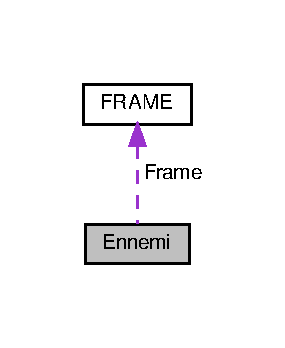
\includegraphics[width=137pt]{structEnnemi__coll__graph}
\end{center}
\end{figure}
\subsection*{Public Attributes}
\begin{DoxyCompactItemize}
\item 
S\+D\+L\+\_\+\+Surface $\ast$ \hyperlink{structEnnemi_aaa6f9be660b13c562cc72213abe89c92}{image}
\item 
S\+D\+L\+\_\+\+Rect \hyperlink{structEnnemi_af8e655f0f8f0c06f87c449550d464e1a}{position\+Animation} \mbox{[}\hyperlink{defs_8h_a5fcf3661be891bf3ecb5c3b0e8489a1b}{S\+P\+R\+I\+T\+E\+\_\+\+E\+N\+N\+E\+M\+I\+\_\+\+NbL}\mbox{]}\mbox{[}\hyperlink{defs_8h_aed42758993e14b4e7f601777bebea3ef}{S\+P\+R\+I\+T\+E\+\_\+\+E\+N\+N\+E\+M\+I\+\_\+\+Nb\+Col}\mbox{]}
\item 
\hyperlink{structFRAME}{F\+R\+A\+ME} \hyperlink{structEnnemi_aacc26f2351740140dcc6727b8aac5492}{Frame}
\item 
S\+D\+L\+\_\+\+Rect \hyperlink{structEnnemi_a38314184da044b6e4a8e9f96775bd94c}{position\+Absolue}
\item 
int \hyperlink{structEnnemi_a9204a1743e29170ed6ae990a07e3980a}{Direction}
\item 
\hyperlink{ennemi_8h_a275a67132f10277ada3a0ee3d616b647}{S\+T\+A\+TE} \hyperlink{structEnnemi_ae860384c5289844a9076ca5d45ebc967}{State}
\end{DoxyCompactItemize}


\subsection{Member Data Documentation}
\mbox{\Hypertarget{structEnnemi_a9204a1743e29170ed6ae990a07e3980a}\label{structEnnemi_a9204a1743e29170ed6ae990a07e3980a}} 
\index{Ennemi@{Ennemi}!Direction@{Direction}}
\index{Direction@{Direction}!Ennemi@{Ennemi}}
\subsubsection{\texorpdfstring{Direction}{Direction}}
{\footnotesize\ttfamily int Ennemi\+::\+Direction}

\mbox{\Hypertarget{structEnnemi_aacc26f2351740140dcc6727b8aac5492}\label{structEnnemi_aacc26f2351740140dcc6727b8aac5492}} 
\index{Ennemi@{Ennemi}!Frame@{Frame}}
\index{Frame@{Frame}!Ennemi@{Ennemi}}
\subsubsection{\texorpdfstring{Frame}{Frame}}
{\footnotesize\ttfamily \hyperlink{structFRAME}{F\+R\+A\+ME} Ennemi\+::\+Frame}

\mbox{\Hypertarget{structEnnemi_aaa6f9be660b13c562cc72213abe89c92}\label{structEnnemi_aaa6f9be660b13c562cc72213abe89c92}} 
\index{Ennemi@{Ennemi}!image@{image}}
\index{image@{image}!Ennemi@{Ennemi}}
\subsubsection{\texorpdfstring{image}{image}}
{\footnotesize\ttfamily S\+D\+L\+\_\+\+Surface$\ast$ Ennemi\+::image}

\mbox{\Hypertarget{structEnnemi_a38314184da044b6e4a8e9f96775bd94c}\label{structEnnemi_a38314184da044b6e4a8e9f96775bd94c}} 
\index{Ennemi@{Ennemi}!position\+Absolue@{position\+Absolue}}
\index{position\+Absolue@{position\+Absolue}!Ennemi@{Ennemi}}
\subsubsection{\texorpdfstring{position\+Absolue}{positionAbsolue}}
{\footnotesize\ttfamily S\+D\+L\+\_\+\+Rect Ennemi\+::position\+Absolue}

\mbox{\Hypertarget{structEnnemi_af8e655f0f8f0c06f87c449550d464e1a}\label{structEnnemi_af8e655f0f8f0c06f87c449550d464e1a}} 
\index{Ennemi@{Ennemi}!position\+Animation@{position\+Animation}}
\index{position\+Animation@{position\+Animation}!Ennemi@{Ennemi}}
\subsubsection{\texorpdfstring{position\+Animation}{positionAnimation}}
{\footnotesize\ttfamily S\+D\+L\+\_\+\+Rect Ennemi\+::position\+Animation\mbox{[}\hyperlink{defs_8h_a5fcf3661be891bf3ecb5c3b0e8489a1b}{S\+P\+R\+I\+T\+E\+\_\+\+E\+N\+N\+E\+M\+I\+\_\+\+NbL}\mbox{]}\mbox{[}\hyperlink{defs_8h_aed42758993e14b4e7f601777bebea3ef}{S\+P\+R\+I\+T\+E\+\_\+\+E\+N\+N\+E\+M\+I\+\_\+\+Nb\+Col}\mbox{]}}

\mbox{\Hypertarget{structEnnemi_ae860384c5289844a9076ca5d45ebc967}\label{structEnnemi_ae860384c5289844a9076ca5d45ebc967}} 
\index{Ennemi@{Ennemi}!State@{State}}
\index{State@{State}!Ennemi@{Ennemi}}
\subsubsection{\texorpdfstring{State}{State}}
{\footnotesize\ttfamily \hyperlink{ennemi_8h_a275a67132f10277ada3a0ee3d616b647}{S\+T\+A\+TE} Ennemi\+::\+State}



The documentation for this struct was generated from the following file\+:\begin{DoxyCompactItemize}
\item 
\hyperlink{ennemi_8h}{ennemi.\+h}\end{DoxyCompactItemize}

\hypertarget{structFRAME}{}\section{F\+R\+A\+ME Struct Reference}
\label{structFRAME}\index{F\+R\+A\+ME@{F\+R\+A\+ME}}


{\ttfamily \#include $<$defs.\+h$>$}

\subsection*{Public Attributes}
\begin{DoxyCompactItemize}
\item 
int \hyperlink{structFRAME_af3ff197cc71e2f1bda04a235cdbff246}{i}
\item 
int \hyperlink{structFRAME_a7aeed9ddb6d33a04d1d11bd59af7ed94}{j}
\end{DoxyCompactItemize}


\subsection{Member Data Documentation}
\mbox{\Hypertarget{structFRAME_af3ff197cc71e2f1bda04a235cdbff246}\label{structFRAME_af3ff197cc71e2f1bda04a235cdbff246}} 
\index{F\+R\+A\+ME@{F\+R\+A\+ME}!i@{i}}
\index{i@{i}!F\+R\+A\+ME@{F\+R\+A\+ME}}
\subsubsection{\texorpdfstring{i}{i}}
{\footnotesize\ttfamily int F\+R\+A\+M\+E\+::i}

\mbox{\Hypertarget{structFRAME_a7aeed9ddb6d33a04d1d11bd59af7ed94}\label{structFRAME_a7aeed9ddb6d33a04d1d11bd59af7ed94}} 
\index{F\+R\+A\+ME@{F\+R\+A\+ME}!j@{j}}
\index{j@{j}!F\+R\+A\+ME@{F\+R\+A\+ME}}
\subsubsection{\texorpdfstring{j}{j}}
{\footnotesize\ttfamily int F\+R\+A\+M\+E\+::j}



The documentation for this struct was generated from the following file\+:\begin{DoxyCompactItemize}
\item 
\hyperlink{defs_8h}{defs.\+h}\end{DoxyCompactItemize}

\hypertarget{structhero}{}\section{hero Struct Reference}
\label{structhero}\index{hero@{hero}}


{\ttfamily \#include $<$hero.\+h$>$}



Collaboration diagram for hero\+:\nopagebreak
\begin{figure}[H]
\begin{center}
\leavevmode
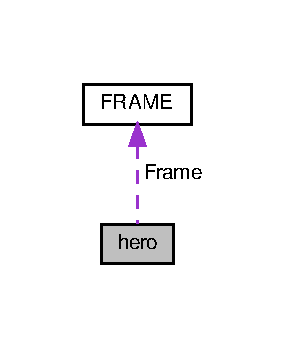
\includegraphics[width=137pt]{structhero__coll__graph}
\end{center}
\end{figure}
\subsection*{Public Attributes}
\begin{DoxyCompactItemize}
\item 
S\+D\+L\+\_\+\+Surface $\ast$ \hyperlink{structhero_aed2e9c21cff3178bfb3253b278221f5d}{image}
\item 
S\+D\+L\+\_\+\+Rect \hyperlink{structhero_a7e9b84755093a175ee262d43911d267a}{position\+Animation} \mbox{[}\hyperlink{defs_8h_ae70e0edee476cfe7672e361c7883c2c3}{S\+P\+R\+I\+T\+E\+\_\+\+H\+E\+R\+O\+\_\+\+NbL}\mbox{]}\mbox{[}\hyperlink{defs_8h_acef7d9709f30d0ebb21fa325bd27a90d}{S\+P\+R\+I\+T\+E\+\_\+\+H\+E\+R\+O\+\_\+\+Nb\+Col}\mbox{]}
\item 
\hyperlink{structFRAME}{F\+R\+A\+ME} \hyperlink{structhero_a5c0232e4390f7b0a64ab38f2fd0aa09b}{Frame}
\item 
S\+D\+L\+\_\+\+Rect \hyperlink{structhero_abda17b4c734008f7324f196824f0ecaf}{position\+Absolue}
\item 
int \hyperlink{structhero_a3bfdfabb0cc2c40d7144ba899a22bc7b}{vies}
\item 
int \hyperlink{structhero_a550bb6de077fc72e5f8c79ba86ea19ac}{is\+\_\+attacking}
\end{DoxyCompactItemize}


\subsection{Member Data Documentation}
\mbox{\Hypertarget{structhero_a5c0232e4390f7b0a64ab38f2fd0aa09b}\label{structhero_a5c0232e4390f7b0a64ab38f2fd0aa09b}} 
\index{hero@{hero}!Frame@{Frame}}
\index{Frame@{Frame}!hero@{hero}}
\subsubsection{\texorpdfstring{Frame}{Frame}}
{\footnotesize\ttfamily \hyperlink{structFRAME}{F\+R\+A\+ME} hero\+::\+Frame}

\mbox{\Hypertarget{structhero_aed2e9c21cff3178bfb3253b278221f5d}\label{structhero_aed2e9c21cff3178bfb3253b278221f5d}} 
\index{hero@{hero}!image@{image}}
\index{image@{image}!hero@{hero}}
\subsubsection{\texorpdfstring{image}{image}}
{\footnotesize\ttfamily S\+D\+L\+\_\+\+Surface$\ast$ hero\+::image}

\mbox{\Hypertarget{structhero_a550bb6de077fc72e5f8c79ba86ea19ac}\label{structhero_a550bb6de077fc72e5f8c79ba86ea19ac}} 
\index{hero@{hero}!is\+\_\+attacking@{is\+\_\+attacking}}
\index{is\+\_\+attacking@{is\+\_\+attacking}!hero@{hero}}
\subsubsection{\texorpdfstring{is\+\_\+attacking}{is\_attacking}}
{\footnotesize\ttfamily int hero\+::is\+\_\+attacking}

\mbox{\Hypertarget{structhero_abda17b4c734008f7324f196824f0ecaf}\label{structhero_abda17b4c734008f7324f196824f0ecaf}} 
\index{hero@{hero}!position\+Absolue@{position\+Absolue}}
\index{position\+Absolue@{position\+Absolue}!hero@{hero}}
\subsubsection{\texorpdfstring{position\+Absolue}{positionAbsolue}}
{\footnotesize\ttfamily S\+D\+L\+\_\+\+Rect hero\+::position\+Absolue}

\mbox{\Hypertarget{structhero_a7e9b84755093a175ee262d43911d267a}\label{structhero_a7e9b84755093a175ee262d43911d267a}} 
\index{hero@{hero}!position\+Animation@{position\+Animation}}
\index{position\+Animation@{position\+Animation}!hero@{hero}}
\subsubsection{\texorpdfstring{position\+Animation}{positionAnimation}}
{\footnotesize\ttfamily S\+D\+L\+\_\+\+Rect hero\+::position\+Animation\mbox{[}\hyperlink{defs_8h_ae70e0edee476cfe7672e361c7883c2c3}{S\+P\+R\+I\+T\+E\+\_\+\+H\+E\+R\+O\+\_\+\+NbL}\mbox{]}\mbox{[}\hyperlink{defs_8h_acef7d9709f30d0ebb21fa325bd27a90d}{S\+P\+R\+I\+T\+E\+\_\+\+H\+E\+R\+O\+\_\+\+Nb\+Col}\mbox{]}}

\mbox{\Hypertarget{structhero_a3bfdfabb0cc2c40d7144ba899a22bc7b}\label{structhero_a3bfdfabb0cc2c40d7144ba899a22bc7b}} 
\index{hero@{hero}!vies@{vies}}
\index{vies@{vies}!hero@{hero}}
\subsubsection{\texorpdfstring{vies}{vies}}
{\footnotesize\ttfamily int hero\+::vies}



The documentation for this struct was generated from the following file\+:\begin{DoxyCompactItemize}
\item 
\hyperlink{hero_8h}{hero.\+h}\end{DoxyCompactItemize}

\hypertarget{structtext}{}\section{text Struct Reference}
\label{structtext}\index{text@{text}}


{\ttfamily \#include $<$text.\+h$>$}

\subsection*{Public Attributes}
\begin{DoxyCompactItemize}
\item 
S\+D\+L\+\_\+\+Rect \hyperlink{structtext_a01cc24369eccbe9ccb68af9a748315d3}{position\+Text}
\item 
char \hyperlink{structtext_afd7610607c0ade6ed450f86e275ddce5}{txt} \mbox{[}20\mbox{]}
\item 
S\+D\+L\+\_\+\+Color \hyperlink{structtext_a0f3134d4dbc64c9b28fa625fb627f9c5}{couleur\+Txt}
\item 
S\+D\+L\+\_\+\+Color \hyperlink{structtext_ae2c25de3d806d9d99afca8d5d41cc4c4}{couleur\+Shadow}
\item 
T\+T\+F\+\_\+\+Font $\ast$ \hyperlink{structtext_aec9ba02a1c093b1db8aa0f16ac092459}{police}
\end{DoxyCompactItemize}


\subsection{Member Data Documentation}
\mbox{\Hypertarget{structtext_ae2c25de3d806d9d99afca8d5d41cc4c4}\label{structtext_ae2c25de3d806d9d99afca8d5d41cc4c4}} 
\index{text@{text}!couleur\+Shadow@{couleur\+Shadow}}
\index{couleur\+Shadow@{couleur\+Shadow}!text@{text}}
\subsubsection{\texorpdfstring{couleur\+Shadow}{couleurShadow}}
{\footnotesize\ttfamily S\+D\+L\+\_\+\+Color text\+::couleur\+Shadow}

\mbox{\Hypertarget{structtext_a0f3134d4dbc64c9b28fa625fb627f9c5}\label{structtext_a0f3134d4dbc64c9b28fa625fb627f9c5}} 
\index{text@{text}!couleur\+Txt@{couleur\+Txt}}
\index{couleur\+Txt@{couleur\+Txt}!text@{text}}
\subsubsection{\texorpdfstring{couleur\+Txt}{couleurTxt}}
{\footnotesize\ttfamily S\+D\+L\+\_\+\+Color text\+::couleur\+Txt}

\mbox{\Hypertarget{structtext_aec9ba02a1c093b1db8aa0f16ac092459}\label{structtext_aec9ba02a1c093b1db8aa0f16ac092459}} 
\index{text@{text}!police@{police}}
\index{police@{police}!text@{text}}
\subsubsection{\texorpdfstring{police}{police}}
{\footnotesize\ttfamily T\+T\+F\+\_\+\+Font$\ast$ text\+::police}

\mbox{\Hypertarget{structtext_a01cc24369eccbe9ccb68af9a748315d3}\label{structtext_a01cc24369eccbe9ccb68af9a748315d3}} 
\index{text@{text}!position\+Text@{position\+Text}}
\index{position\+Text@{position\+Text}!text@{text}}
\subsubsection{\texorpdfstring{position\+Text}{positionText}}
{\footnotesize\ttfamily S\+D\+L\+\_\+\+Rect text\+::position\+Text}

\mbox{\Hypertarget{structtext_afd7610607c0ade6ed450f86e275ddce5}\label{structtext_afd7610607c0ade6ed450f86e275ddce5}} 
\index{text@{text}!txt@{txt}}
\index{txt@{txt}!text@{text}}
\subsubsection{\texorpdfstring{txt}{txt}}
{\footnotesize\ttfamily char text\+::txt\mbox{[}20\mbox{]}}



The documentation for this struct was generated from the following file\+:\begin{DoxyCompactItemize}
\item 
\hyperlink{text_8h}{text.\+h}\end{DoxyCompactItemize}

\chapter{File Documentation}
\hypertarget{background_8c}{}\section{background.\+c File Reference}
\label{background_8c}\index{background.\+c@{background.\+c}}
{\ttfamily \#include $<$S\+D\+L/\+S\+D\+L\+\_\+image.\+h$>$}\newline
{\ttfamily \#include \char`\"{}background.\+h\char`\"{}}\newline
Include dependency graph for background.\+c\+:
\nopagebreak
\begin{figure}[H]
\begin{center}
\leavevmode
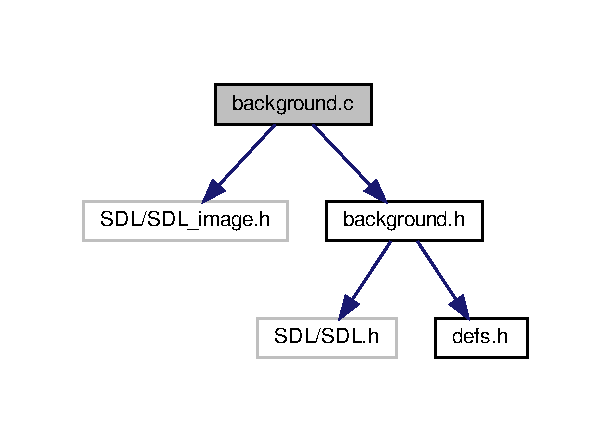
\includegraphics[width=293pt]{background_8c__incl}
\end{center}
\end{figure}
\subsection*{Functions}
\begin{DoxyCompactItemize}
\item 
int \hyperlink{background_8c_a64f4f98a94abc44908b52e952c05664d}{init\+\_\+background} (\hyperlink{structBackground}{Background} $\ast$B, char $\ast$path, \hyperlink{structBackground}{Background} $\ast$B2)
\item 
int \hyperlink{background_8c_aa4bc88437f80ec463c6a370db7bc7adb}{load\+Background} (\hyperlink{structBackground}{Background} $\ast$Backg, char $\ast$path, \hyperlink{structBackground}{Background} $\ast$Backg2)
\item 
void \hyperlink{background_8c_a0a466aed05d60587c8430110812f68be}{init\+Backgound\+Attributes} (\hyperlink{structBackground}{Background} $\ast$Backg, \hyperlink{structBackground}{Background} $\ast$Backg2)
\item 
void \hyperlink{background_8c_a80a77e36e17fc60ff6671f447363a05e}{display\+\_\+background} (\hyperlink{structBackground}{Background} Backg, \hyperlink{structBackground}{Background} Backg2, S\+D\+L\+\_\+\+Surface $\ast$screen)
\item 
void \hyperlink{background_8c_ab5e1830996c2c32cc4860e2321a22b76}{free\+Background} (\hyperlink{structBackground}{Background} $\ast$Backg, \hyperlink{structBackground}{Background} $\ast$Backg2)
\end{DoxyCompactItemize}


\subsection{Function Documentation}
\mbox{\Hypertarget{background_8c_a80a77e36e17fc60ff6671f447363a05e}\label{background_8c_a80a77e36e17fc60ff6671f447363a05e}} 
\index{background.\+c@{background.\+c}!display\+\_\+background@{display\+\_\+background}}
\index{display\+\_\+background@{display\+\_\+background}!background.\+c@{background.\+c}}
\subsubsection{\texorpdfstring{display\+\_\+background()}{display\_background()}}
{\footnotesize\ttfamily void display\+\_\+background (\begin{DoxyParamCaption}\item[{\hyperlink{structBackground}{Background}}]{Backg,  }\item[{\hyperlink{structBackground}{Background}}]{Backg2,  }\item[{S\+D\+L\+\_\+\+Surface $\ast$}]{screen }\end{DoxyParamCaption})}

Here is the caller graph for this function\+:
\nopagebreak
\begin{figure}[H]
\begin{center}
\leavevmode
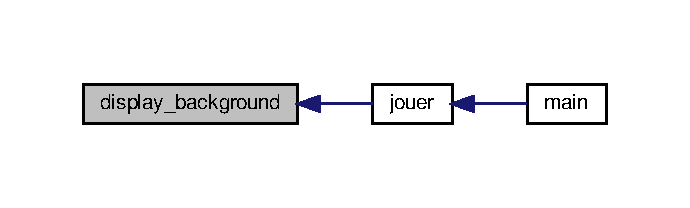
\includegraphics[width=331pt]{background_8c_a80a77e36e17fc60ff6671f447363a05e_icgraph}
\end{center}
\end{figure}
\mbox{\Hypertarget{background_8c_ab5e1830996c2c32cc4860e2321a22b76}\label{background_8c_ab5e1830996c2c32cc4860e2321a22b76}} 
\index{background.\+c@{background.\+c}!free\+Background@{free\+Background}}
\index{free\+Background@{free\+Background}!background.\+c@{background.\+c}}
\subsubsection{\texorpdfstring{free\+Background()}{freeBackground()}}
{\footnotesize\ttfamily void free\+Background (\begin{DoxyParamCaption}\item[{\hyperlink{structBackground}{Background} $\ast$}]{Backg,  }\item[{\hyperlink{structBackground}{Background} $\ast$}]{Backg2 }\end{DoxyParamCaption})}

Here is the caller graph for this function\+:
\nopagebreak
\begin{figure}[H]
\begin{center}
\leavevmode
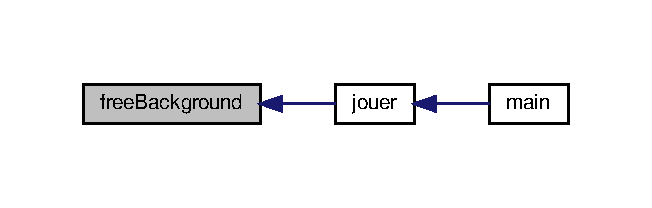
\includegraphics[width=313pt]{background_8c_ab5e1830996c2c32cc4860e2321a22b76_icgraph}
\end{center}
\end{figure}
\mbox{\Hypertarget{background_8c_a64f4f98a94abc44908b52e952c05664d}\label{background_8c_a64f4f98a94abc44908b52e952c05664d}} 
\index{background.\+c@{background.\+c}!init\+\_\+background@{init\+\_\+background}}
\index{init\+\_\+background@{init\+\_\+background}!background.\+c@{background.\+c}}
\subsubsection{\texorpdfstring{init\+\_\+background()}{init\_background()}}
{\footnotesize\ttfamily int init\+\_\+background (\begin{DoxyParamCaption}\item[{\hyperlink{structBackground}{Background} $\ast$}]{B,  }\item[{char $\ast$}]{path,  }\item[{\hyperlink{structBackground}{Background} $\ast$}]{B2 }\end{DoxyParamCaption})}

Here is the call graph for this function\+:
\nopagebreak
\begin{figure}[H]
\begin{center}
\leavevmode
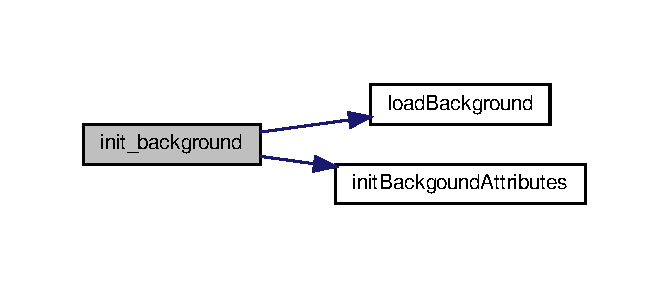
\includegraphics[width=321pt]{background_8c_a64f4f98a94abc44908b52e952c05664d_cgraph}
\end{center}
\end{figure}
Here is the caller graph for this function\+:
\nopagebreak
\begin{figure}[H]
\begin{center}
\leavevmode
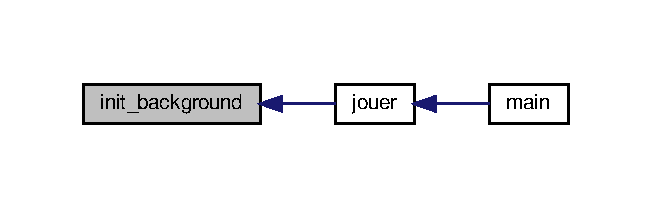
\includegraphics[width=313pt]{background_8c_a64f4f98a94abc44908b52e952c05664d_icgraph}
\end{center}
\end{figure}
\mbox{\Hypertarget{background_8c_a0a466aed05d60587c8430110812f68be}\label{background_8c_a0a466aed05d60587c8430110812f68be}} 
\index{background.\+c@{background.\+c}!init\+Backgound\+Attributes@{init\+Backgound\+Attributes}}
\index{init\+Backgound\+Attributes@{init\+Backgound\+Attributes}!background.\+c@{background.\+c}}
\subsubsection{\texorpdfstring{init\+Backgound\+Attributes()}{initBackgoundAttributes()}}
{\footnotesize\ttfamily void init\+Backgound\+Attributes (\begin{DoxyParamCaption}\item[{\hyperlink{structBackground}{Background} $\ast$}]{Backg,  }\item[{\hyperlink{structBackground}{Background} $\ast$}]{Backg2 }\end{DoxyParamCaption})}

Here is the caller graph for this function\+:
\nopagebreak
\begin{figure}[H]
\begin{center}
\leavevmode
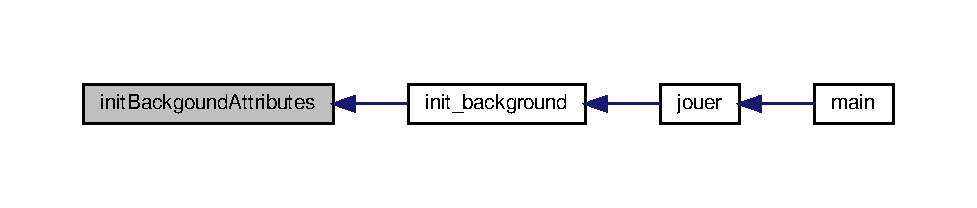
\includegraphics[width=350pt]{background_8c_a0a466aed05d60587c8430110812f68be_icgraph}
\end{center}
\end{figure}
\mbox{\Hypertarget{background_8c_aa4bc88437f80ec463c6a370db7bc7adb}\label{background_8c_aa4bc88437f80ec463c6a370db7bc7adb}} 
\index{background.\+c@{background.\+c}!load\+Background@{load\+Background}}
\index{load\+Background@{load\+Background}!background.\+c@{background.\+c}}
\subsubsection{\texorpdfstring{load\+Background()}{loadBackground()}}
{\footnotesize\ttfamily int load\+Background (\begin{DoxyParamCaption}\item[{\hyperlink{structBackground}{Background} $\ast$}]{Backg,  }\item[{char $\ast$}]{path,  }\item[{\hyperlink{structBackground}{Background} $\ast$}]{Backg2 }\end{DoxyParamCaption})}

Here is the caller graph for this function\+:
\nopagebreak
\begin{figure}[H]
\begin{center}
\leavevmode
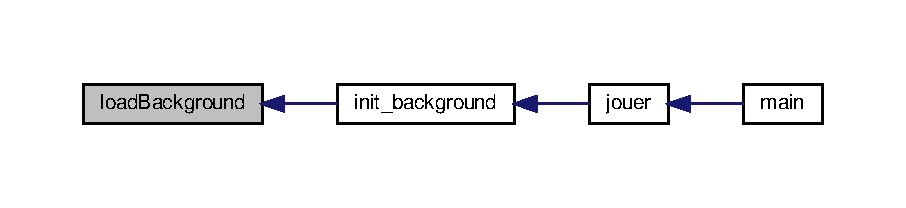
\includegraphics[width=350pt]{background_8c_aa4bc88437f80ec463c6a370db7bc7adb_icgraph}
\end{center}
\end{figure}

\hypertarget{background_8h}{}\section{background.\+h File Reference}
\label{background_8h}\index{background.\+h@{background.\+h}}
{\ttfamily \#include $<$S\+D\+L/\+S\+D\+L.\+h$>$}\newline
{\ttfamily \#include \char`\"{}defs.\+h\char`\"{}}\newline
Include dependency graph for background.\+h\+:
\nopagebreak
\begin{figure}[H]
\begin{center}
\leavevmode
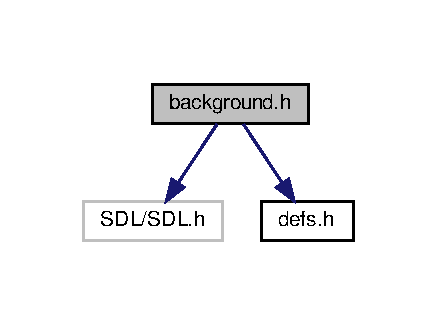
\includegraphics[width=210pt]{background_8h__incl}
\end{center}
\end{figure}
This graph shows which files directly or indirectly include this file\+:
\nopagebreak
\begin{figure}[H]
\begin{center}
\leavevmode
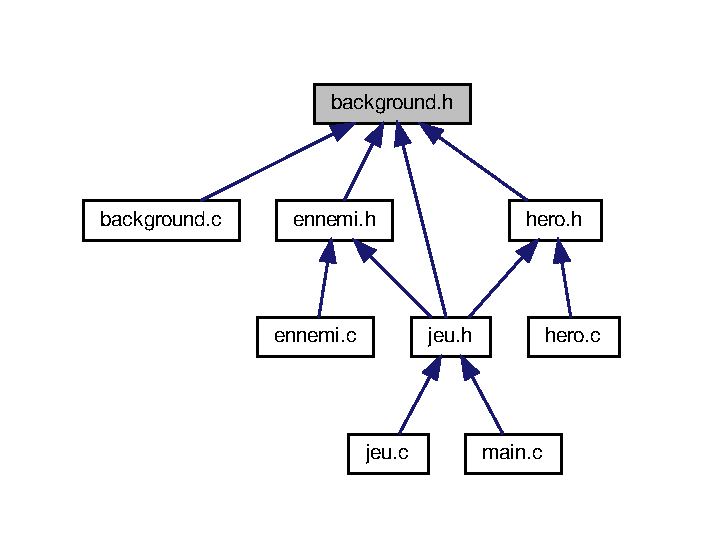
\includegraphics[width=338pt]{background_8h__dep__incl}
\end{center}
\end{figure}
\subsection*{Classes}
\begin{DoxyCompactItemize}
\item 
struct \hyperlink{structBackground}{Background}
\end{DoxyCompactItemize}
\subsection*{Typedefs}
\begin{DoxyCompactItemize}
\item 
typedef struct \hyperlink{structBackground}{Background} \hyperlink{background_8h_add827aeea72432201c9e671c74d7b4dd}{Background}
\end{DoxyCompactItemize}
\subsection*{Functions}
\begin{DoxyCompactItemize}
\item 
int \hyperlink{background_8h_a64f4f98a94abc44908b52e952c05664d}{init\+\_\+background} (\hyperlink{structBackground}{Background} $\ast$B, char $\ast$path, \hyperlink{structBackground}{Background} $\ast$B2)
\item 
void \hyperlink{background_8h_a2a4e3af025d5c6f26f13674e8e5db9a9}{display\+\_\+background} (\hyperlink{structBackground}{Background} B, \hyperlink{structBackground}{Background} B2, S\+D\+L\+\_\+\+Surface $\ast$screen)
\item 
void \hyperlink{background_8h_a009d33c2574a26f1f317a685a4a877a1}{free\+Background} (\hyperlink{structBackground}{Background} $\ast$B, \hyperlink{structBackground}{Background} $\ast$B2)
\item 
int \hyperlink{background_8h_a60583485d12efdb7ab36240ae7805f77}{load\+Background} (\hyperlink{structBackground}{Background} $\ast$B, char $\ast$path, \hyperlink{structBackground}{Background} $\ast$B2)
\item 
void \hyperlink{background_8h_adb52c66b1abec6c8aa921e5e743ae65a}{init\+Backgound\+Attributes} (\hyperlink{structBackground}{Background} $\ast$B, \hyperlink{structBackground}{Background} $\ast$B2)
\end{DoxyCompactItemize}


\subsection{Typedef Documentation}
\mbox{\Hypertarget{background_8h_add827aeea72432201c9e671c74d7b4dd}\label{background_8h_add827aeea72432201c9e671c74d7b4dd}} 
\index{background.\+h@{background.\+h}!Background@{Background}}
\index{Background@{Background}!background.\+h@{background.\+h}}
\subsubsection{\texorpdfstring{Background}{Background}}
{\footnotesize\ttfamily typedef struct \hyperlink{structBackground}{Background} \hyperlink{structBackground}{Background}}



\subsection{Function Documentation}
\mbox{\Hypertarget{background_8h_a2a4e3af025d5c6f26f13674e8e5db9a9}\label{background_8h_a2a4e3af025d5c6f26f13674e8e5db9a9}} 
\index{background.\+h@{background.\+h}!display\+\_\+background@{display\+\_\+background}}
\index{display\+\_\+background@{display\+\_\+background}!background.\+h@{background.\+h}}
\subsubsection{\texorpdfstring{display\+\_\+background()}{display\_background()}}
{\footnotesize\ttfamily void display\+\_\+background (\begin{DoxyParamCaption}\item[{\hyperlink{structBackground}{Background}}]{B,  }\item[{\hyperlink{structBackground}{Background}}]{B2,  }\item[{S\+D\+L\+\_\+\+Surface $\ast$}]{screen }\end{DoxyParamCaption})}

Here is the caller graph for this function\+:
\nopagebreak
\begin{figure}[H]
\begin{center}
\leavevmode
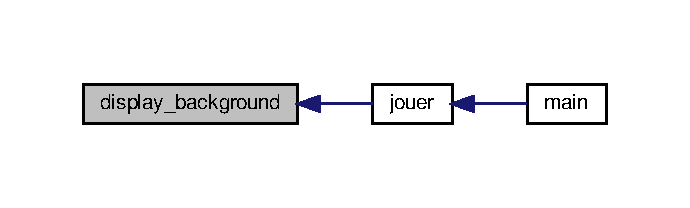
\includegraphics[width=331pt]{background_8h_a2a4e3af025d5c6f26f13674e8e5db9a9_icgraph}
\end{center}
\end{figure}
\mbox{\Hypertarget{background_8h_a009d33c2574a26f1f317a685a4a877a1}\label{background_8h_a009d33c2574a26f1f317a685a4a877a1}} 
\index{background.\+h@{background.\+h}!free\+Background@{free\+Background}}
\index{free\+Background@{free\+Background}!background.\+h@{background.\+h}}
\subsubsection{\texorpdfstring{free\+Background()}{freeBackground()}}
{\footnotesize\ttfamily void free\+Background (\begin{DoxyParamCaption}\item[{\hyperlink{structBackground}{Background} $\ast$}]{B,  }\item[{\hyperlink{structBackground}{Background} $\ast$}]{B2 }\end{DoxyParamCaption})}

Here is the caller graph for this function\+:
\nopagebreak
\begin{figure}[H]
\begin{center}
\leavevmode
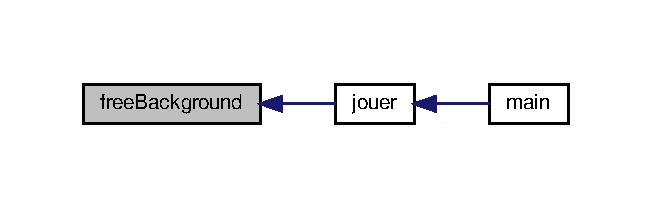
\includegraphics[width=313pt]{background_8h_a009d33c2574a26f1f317a685a4a877a1_icgraph}
\end{center}
\end{figure}
\mbox{\Hypertarget{background_8h_a64f4f98a94abc44908b52e952c05664d}\label{background_8h_a64f4f98a94abc44908b52e952c05664d}} 
\index{background.\+h@{background.\+h}!init\+\_\+background@{init\+\_\+background}}
\index{init\+\_\+background@{init\+\_\+background}!background.\+h@{background.\+h}}
\subsubsection{\texorpdfstring{init\+\_\+background()}{init\_background()}}
{\footnotesize\ttfamily int init\+\_\+background (\begin{DoxyParamCaption}\item[{\hyperlink{structBackground}{Background} $\ast$}]{B,  }\item[{char $\ast$}]{path,  }\item[{\hyperlink{structBackground}{Background} $\ast$}]{B2 }\end{DoxyParamCaption})}

Here is the call graph for this function\+:
\nopagebreak
\begin{figure}[H]
\begin{center}
\leavevmode
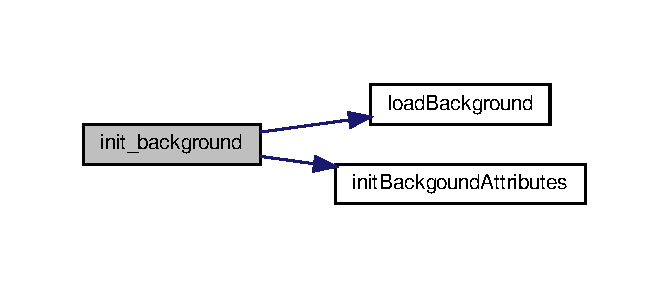
\includegraphics[width=321pt]{background_8h_a64f4f98a94abc44908b52e952c05664d_cgraph}
\end{center}
\end{figure}
Here is the caller graph for this function\+:
\nopagebreak
\begin{figure}[H]
\begin{center}
\leavevmode
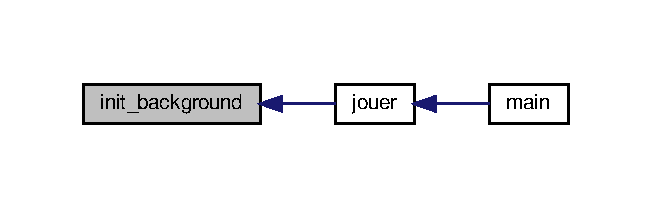
\includegraphics[width=313pt]{background_8h_a64f4f98a94abc44908b52e952c05664d_icgraph}
\end{center}
\end{figure}
\mbox{\Hypertarget{background_8h_adb52c66b1abec6c8aa921e5e743ae65a}\label{background_8h_adb52c66b1abec6c8aa921e5e743ae65a}} 
\index{background.\+h@{background.\+h}!init\+Backgound\+Attributes@{init\+Backgound\+Attributes}}
\index{init\+Backgound\+Attributes@{init\+Backgound\+Attributes}!background.\+h@{background.\+h}}
\subsubsection{\texorpdfstring{init\+Backgound\+Attributes()}{initBackgoundAttributes()}}
{\footnotesize\ttfamily void init\+Backgound\+Attributes (\begin{DoxyParamCaption}\item[{\hyperlink{structBackground}{Background} $\ast$}]{B,  }\item[{\hyperlink{structBackground}{Background} $\ast$}]{B2 }\end{DoxyParamCaption})}

Here is the caller graph for this function\+:
\nopagebreak
\begin{figure}[H]
\begin{center}
\leavevmode
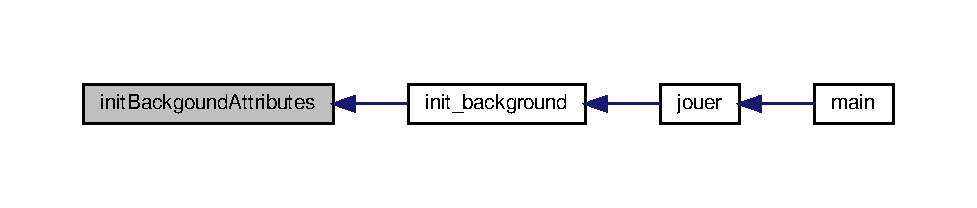
\includegraphics[width=350pt]{background_8h_adb52c66b1abec6c8aa921e5e743ae65a_icgraph}
\end{center}
\end{figure}
\mbox{\Hypertarget{background_8h_a60583485d12efdb7ab36240ae7805f77}\label{background_8h_a60583485d12efdb7ab36240ae7805f77}} 
\index{background.\+h@{background.\+h}!load\+Background@{load\+Background}}
\index{load\+Background@{load\+Background}!background.\+h@{background.\+h}}
\subsubsection{\texorpdfstring{load\+Background()}{loadBackground()}}
{\footnotesize\ttfamily int load\+Background (\begin{DoxyParamCaption}\item[{\hyperlink{structBackground}{Background} $\ast$}]{B,  }\item[{char $\ast$}]{path,  }\item[{\hyperlink{structBackground}{Background} $\ast$}]{B2 }\end{DoxyParamCaption})}

Here is the caller graph for this function\+:
\nopagebreak
\begin{figure}[H]
\begin{center}
\leavevmode
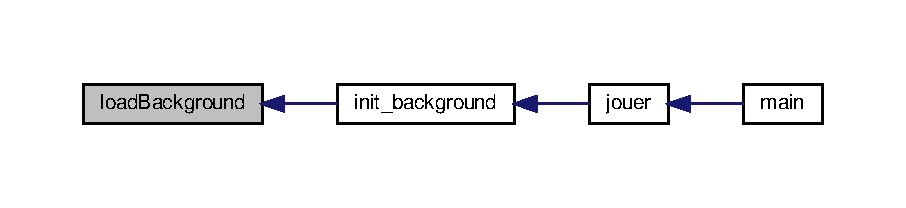
\includegraphics[width=350pt]{background_8h_a60583485d12efdb7ab36240ae7805f77_icgraph}
\end{center}
\end{figure}

\hypertarget{defs_8h}{}\section{defs.\+h File Reference}
\label{defs_8h}\index{defs.\+h@{defs.\+h}}
This graph shows which files directly or indirectly include this file\+:
\nopagebreak
\begin{figure}[H]
\begin{center}
\leavevmode
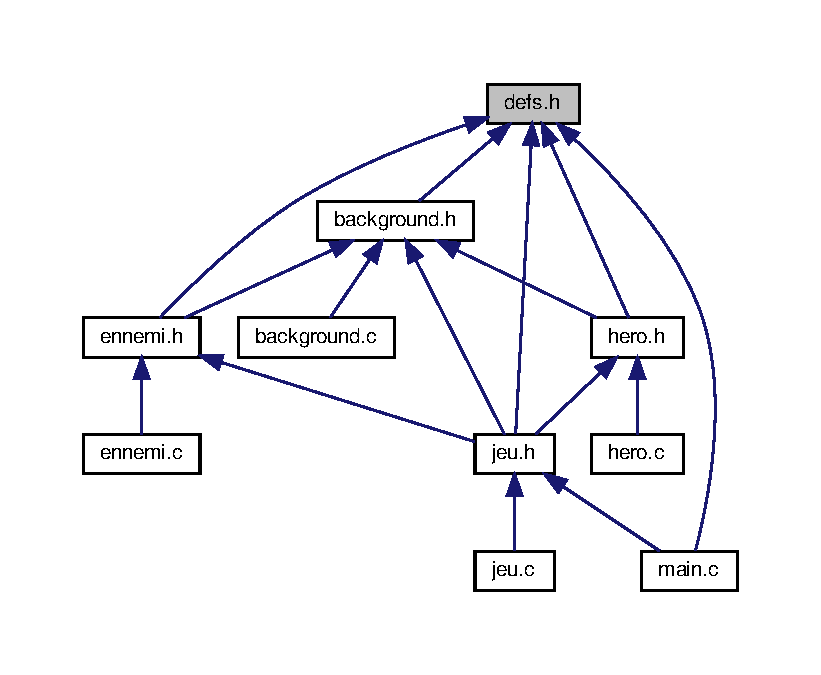
\includegraphics[width=350pt]{defs_8h__dep__incl}
\end{center}
\end{figure}
\subsection*{Classes}
\begin{DoxyCompactItemize}
\item 
struct \hyperlink{structFRAME}{F\+R\+A\+ME}
\end{DoxyCompactItemize}
\subsection*{Macros}
\begin{DoxyCompactItemize}
\item 
\#define \hyperlink{defs_8h_a99e395e0c0dfe9c75e5d95d715f361c5}{waiting}~1
\item 
\#define \hyperlink{defs_8h_a051bdf409f5cdcdfb2d9e636c492804b}{following}~2
\item 
\#define \hyperlink{defs_8h_a12dd7bcfe5d870c3228f2f7c469f787a}{attack}~3
\item 
\#define \hyperlink{defs_8h_aef7744d055365568a5141d19998d9bc1}{B\+A\+C\+K\+G\+N\+D\+\_\+W}~1600
\item 
\#define \hyperlink{defs_8h_a34f06e62293685db0481ef3f01b53d5b}{B\+A\+C\+K\+G\+N\+D\+\_\+H}~600
\item 
\#define \hyperlink{defs_8h_a9728f27ebcd67564a9c7c690d4743658}{B\+A\+C\+K\+G\+N\+D2\+\_\+W}~1600
\item 
\#define \hyperlink{defs_8h_a756132600a5191097395627ac3b85390}{B\+A\+C\+K\+G\+N\+D2\+\_\+H}~100
\item 
\#define \hyperlink{defs_8h_a668d31b2febcffabdb4a1488b2535bd0}{Hero\+\_\+\+W\+I\+D\+TH}~100
\item 
\#define \hyperlink{defs_8h_aff863547b8bd01face29ac13c114ff48}{Hero\+\_\+\+H\+E\+I\+G\+HT}~100
\item 
\#define \hyperlink{defs_8h_a7e272edc90e62eafd13edd7d6d74897d}{Ennemi\+\_\+\+W\+I\+D\+TH}~100
\item 
\#define \hyperlink{defs_8h_a3845e28887de1ba8ec3acf7b16cb2f22}{Ennemi\+\_\+\+H\+E\+I\+G\+HT}~100
\item 
\#define \hyperlink{defs_8h_a9b6bc9242882d1e758e06ed751a2e8ec}{S\+C\+R\+E\+E\+N\+\_\+W}~1600
\item 
\#define \hyperlink{defs_8h_a27cddfd509d28b4b2b0b44c093fac090}{S\+C\+R\+E\+E\+N\+\_\+H}~600
\item 
\#define \hyperlink{defs_8h_ae70e0edee476cfe7672e361c7883c2c3}{S\+P\+R\+I\+T\+E\+\_\+\+H\+E\+R\+O\+\_\+\+NbL}~4
\item 
\#define \hyperlink{defs_8h_acef7d9709f30d0ebb21fa325bd27a90d}{S\+P\+R\+I\+T\+E\+\_\+\+H\+E\+R\+O\+\_\+\+Nb\+Col}~4
\item 
\#define \hyperlink{defs_8h_a5fcf3661be891bf3ecb5c3b0e8489a1b}{S\+P\+R\+I\+T\+E\+\_\+\+E\+N\+N\+E\+M\+I\+\_\+\+NbL}~4
\item 
\#define \hyperlink{defs_8h_aed42758993e14b4e7f601777bebea3ef}{S\+P\+R\+I\+T\+E\+\_\+\+E\+N\+N\+E\+M\+I\+\_\+\+Nb\+Col}~4
\end{DoxyCompactItemize}
\subsection*{Typedefs}
\begin{DoxyCompactItemize}
\item 
typedef int \hyperlink{defs_8h_a1062901a7428fdd9c7f180f5e01ea056}{bool}
\item 
typedef struct \hyperlink{structFRAME}{F\+R\+A\+ME} \hyperlink{defs_8h_ac4903c07e4309db57fdc2f9dd8af3d54}{F\+R\+A\+ME}
\end{DoxyCompactItemize}
\subsection*{Enumerations}
\begin{DoxyCompactItemize}
\item 
enum \{ \hyperlink{defs_8h_a06fc87d81c62e9abb8790b6e5713c55bae9de385ef6fe9bf3360d1038396b884c}{false}, 
\hyperlink{defs_8h_a06fc87d81c62e9abb8790b6e5713c55ba08f175a5505a10b9ed657defeb050e4b}{true}
 \}
\end{DoxyCompactItemize}


\subsection{Macro Definition Documentation}
\mbox{\Hypertarget{defs_8h_a12dd7bcfe5d870c3228f2f7c469f787a}\label{defs_8h_a12dd7bcfe5d870c3228f2f7c469f787a}} 
\index{defs.\+h@{defs.\+h}!attack@{attack}}
\index{attack@{attack}!defs.\+h@{defs.\+h}}
\subsubsection{\texorpdfstring{attack}{attack}}
{\footnotesize\ttfamily \#define attack~3}

\mbox{\Hypertarget{defs_8h_a756132600a5191097395627ac3b85390}\label{defs_8h_a756132600a5191097395627ac3b85390}} 
\index{defs.\+h@{defs.\+h}!B\+A\+C\+K\+G\+N\+D2\+\_\+H@{B\+A\+C\+K\+G\+N\+D2\+\_\+H}}
\index{B\+A\+C\+K\+G\+N\+D2\+\_\+H@{B\+A\+C\+K\+G\+N\+D2\+\_\+H}!defs.\+h@{defs.\+h}}
\subsubsection{\texorpdfstring{B\+A\+C\+K\+G\+N\+D2\+\_\+H}{BACKGND2\_H}}
{\footnotesize\ttfamily \#define B\+A\+C\+K\+G\+N\+D2\+\_\+H~100}

\mbox{\Hypertarget{defs_8h_a9728f27ebcd67564a9c7c690d4743658}\label{defs_8h_a9728f27ebcd67564a9c7c690d4743658}} 
\index{defs.\+h@{defs.\+h}!B\+A\+C\+K\+G\+N\+D2\+\_\+W@{B\+A\+C\+K\+G\+N\+D2\+\_\+W}}
\index{B\+A\+C\+K\+G\+N\+D2\+\_\+W@{B\+A\+C\+K\+G\+N\+D2\+\_\+W}!defs.\+h@{defs.\+h}}
\subsubsection{\texorpdfstring{B\+A\+C\+K\+G\+N\+D2\+\_\+W}{BACKGND2\_W}}
{\footnotesize\ttfamily \#define B\+A\+C\+K\+G\+N\+D2\+\_\+W~1600}

\mbox{\Hypertarget{defs_8h_a34f06e62293685db0481ef3f01b53d5b}\label{defs_8h_a34f06e62293685db0481ef3f01b53d5b}} 
\index{defs.\+h@{defs.\+h}!B\+A\+C\+K\+G\+N\+D\+\_\+H@{B\+A\+C\+K\+G\+N\+D\+\_\+H}}
\index{B\+A\+C\+K\+G\+N\+D\+\_\+H@{B\+A\+C\+K\+G\+N\+D\+\_\+H}!defs.\+h@{defs.\+h}}
\subsubsection{\texorpdfstring{B\+A\+C\+K\+G\+N\+D\+\_\+H}{BACKGND\_H}}
{\footnotesize\ttfamily \#define B\+A\+C\+K\+G\+N\+D\+\_\+H~600}

\mbox{\Hypertarget{defs_8h_aef7744d055365568a5141d19998d9bc1}\label{defs_8h_aef7744d055365568a5141d19998d9bc1}} 
\index{defs.\+h@{defs.\+h}!B\+A\+C\+K\+G\+N\+D\+\_\+W@{B\+A\+C\+K\+G\+N\+D\+\_\+W}}
\index{B\+A\+C\+K\+G\+N\+D\+\_\+W@{B\+A\+C\+K\+G\+N\+D\+\_\+W}!defs.\+h@{defs.\+h}}
\subsubsection{\texorpdfstring{B\+A\+C\+K\+G\+N\+D\+\_\+W}{BACKGND\_W}}
{\footnotesize\ttfamily \#define B\+A\+C\+K\+G\+N\+D\+\_\+W~1600}

\mbox{\Hypertarget{defs_8h_a3845e28887de1ba8ec3acf7b16cb2f22}\label{defs_8h_a3845e28887de1ba8ec3acf7b16cb2f22}} 
\index{defs.\+h@{defs.\+h}!Ennemi\+\_\+\+H\+E\+I\+G\+HT@{Ennemi\+\_\+\+H\+E\+I\+G\+HT}}
\index{Ennemi\+\_\+\+H\+E\+I\+G\+HT@{Ennemi\+\_\+\+H\+E\+I\+G\+HT}!defs.\+h@{defs.\+h}}
\subsubsection{\texorpdfstring{Ennemi\+\_\+\+H\+E\+I\+G\+HT}{Ennemi\_HEIGHT}}
{\footnotesize\ttfamily \#define Ennemi\+\_\+\+H\+E\+I\+G\+HT~100}

\mbox{\Hypertarget{defs_8h_a7e272edc90e62eafd13edd7d6d74897d}\label{defs_8h_a7e272edc90e62eafd13edd7d6d74897d}} 
\index{defs.\+h@{defs.\+h}!Ennemi\+\_\+\+W\+I\+D\+TH@{Ennemi\+\_\+\+W\+I\+D\+TH}}
\index{Ennemi\+\_\+\+W\+I\+D\+TH@{Ennemi\+\_\+\+W\+I\+D\+TH}!defs.\+h@{defs.\+h}}
\subsubsection{\texorpdfstring{Ennemi\+\_\+\+W\+I\+D\+TH}{Ennemi\_WIDTH}}
{\footnotesize\ttfamily \#define Ennemi\+\_\+\+W\+I\+D\+TH~100}

\mbox{\Hypertarget{defs_8h_a051bdf409f5cdcdfb2d9e636c492804b}\label{defs_8h_a051bdf409f5cdcdfb2d9e636c492804b}} 
\index{defs.\+h@{defs.\+h}!following@{following}}
\index{following@{following}!defs.\+h@{defs.\+h}}
\subsubsection{\texorpdfstring{following}{following}}
{\footnotesize\ttfamily \#define following~2}

\mbox{\Hypertarget{defs_8h_aff863547b8bd01face29ac13c114ff48}\label{defs_8h_aff863547b8bd01face29ac13c114ff48}} 
\index{defs.\+h@{defs.\+h}!Hero\+\_\+\+H\+E\+I\+G\+HT@{Hero\+\_\+\+H\+E\+I\+G\+HT}}
\index{Hero\+\_\+\+H\+E\+I\+G\+HT@{Hero\+\_\+\+H\+E\+I\+G\+HT}!defs.\+h@{defs.\+h}}
\subsubsection{\texorpdfstring{Hero\+\_\+\+H\+E\+I\+G\+HT}{Hero\_HEIGHT}}
{\footnotesize\ttfamily \#define Hero\+\_\+\+H\+E\+I\+G\+HT~100}

\mbox{\Hypertarget{defs_8h_a668d31b2febcffabdb4a1488b2535bd0}\label{defs_8h_a668d31b2febcffabdb4a1488b2535bd0}} 
\index{defs.\+h@{defs.\+h}!Hero\+\_\+\+W\+I\+D\+TH@{Hero\+\_\+\+W\+I\+D\+TH}}
\index{Hero\+\_\+\+W\+I\+D\+TH@{Hero\+\_\+\+W\+I\+D\+TH}!defs.\+h@{defs.\+h}}
\subsubsection{\texorpdfstring{Hero\+\_\+\+W\+I\+D\+TH}{Hero\_WIDTH}}
{\footnotesize\ttfamily \#define Hero\+\_\+\+W\+I\+D\+TH~100}

\mbox{\Hypertarget{defs_8h_a27cddfd509d28b4b2b0b44c093fac090}\label{defs_8h_a27cddfd509d28b4b2b0b44c093fac090}} 
\index{defs.\+h@{defs.\+h}!S\+C\+R\+E\+E\+N\+\_\+H@{S\+C\+R\+E\+E\+N\+\_\+H}}
\index{S\+C\+R\+E\+E\+N\+\_\+H@{S\+C\+R\+E\+E\+N\+\_\+H}!defs.\+h@{defs.\+h}}
\subsubsection{\texorpdfstring{S\+C\+R\+E\+E\+N\+\_\+H}{SCREEN\_H}}
{\footnotesize\ttfamily \#define S\+C\+R\+E\+E\+N\+\_\+H~600}

\mbox{\Hypertarget{defs_8h_a9b6bc9242882d1e758e06ed751a2e8ec}\label{defs_8h_a9b6bc9242882d1e758e06ed751a2e8ec}} 
\index{defs.\+h@{defs.\+h}!S\+C\+R\+E\+E\+N\+\_\+W@{S\+C\+R\+E\+E\+N\+\_\+W}}
\index{S\+C\+R\+E\+E\+N\+\_\+W@{S\+C\+R\+E\+E\+N\+\_\+W}!defs.\+h@{defs.\+h}}
\subsubsection{\texorpdfstring{S\+C\+R\+E\+E\+N\+\_\+W}{SCREEN\_W}}
{\footnotesize\ttfamily \#define S\+C\+R\+E\+E\+N\+\_\+W~1600}

\mbox{\Hypertarget{defs_8h_aed42758993e14b4e7f601777bebea3ef}\label{defs_8h_aed42758993e14b4e7f601777bebea3ef}} 
\index{defs.\+h@{defs.\+h}!S\+P\+R\+I\+T\+E\+\_\+\+E\+N\+N\+E\+M\+I\+\_\+\+Nb\+Col@{S\+P\+R\+I\+T\+E\+\_\+\+E\+N\+N\+E\+M\+I\+\_\+\+Nb\+Col}}
\index{S\+P\+R\+I\+T\+E\+\_\+\+E\+N\+N\+E\+M\+I\+\_\+\+Nb\+Col@{S\+P\+R\+I\+T\+E\+\_\+\+E\+N\+N\+E\+M\+I\+\_\+\+Nb\+Col}!defs.\+h@{defs.\+h}}
\subsubsection{\texorpdfstring{S\+P\+R\+I\+T\+E\+\_\+\+E\+N\+N\+E\+M\+I\+\_\+\+Nb\+Col}{SPRITE\_ENNEMI\_NbCol}}
{\footnotesize\ttfamily \#define S\+P\+R\+I\+T\+E\+\_\+\+E\+N\+N\+E\+M\+I\+\_\+\+Nb\+Col~4}

\mbox{\Hypertarget{defs_8h_a5fcf3661be891bf3ecb5c3b0e8489a1b}\label{defs_8h_a5fcf3661be891bf3ecb5c3b0e8489a1b}} 
\index{defs.\+h@{defs.\+h}!S\+P\+R\+I\+T\+E\+\_\+\+E\+N\+N\+E\+M\+I\+\_\+\+NbL@{S\+P\+R\+I\+T\+E\+\_\+\+E\+N\+N\+E\+M\+I\+\_\+\+NbL}}
\index{S\+P\+R\+I\+T\+E\+\_\+\+E\+N\+N\+E\+M\+I\+\_\+\+NbL@{S\+P\+R\+I\+T\+E\+\_\+\+E\+N\+N\+E\+M\+I\+\_\+\+NbL}!defs.\+h@{defs.\+h}}
\subsubsection{\texorpdfstring{S\+P\+R\+I\+T\+E\+\_\+\+E\+N\+N\+E\+M\+I\+\_\+\+NbL}{SPRITE\_ENNEMI\_NbL}}
{\footnotesize\ttfamily \#define S\+P\+R\+I\+T\+E\+\_\+\+E\+N\+N\+E\+M\+I\+\_\+\+NbL~4}

\mbox{\Hypertarget{defs_8h_acef7d9709f30d0ebb21fa325bd27a90d}\label{defs_8h_acef7d9709f30d0ebb21fa325bd27a90d}} 
\index{defs.\+h@{defs.\+h}!S\+P\+R\+I\+T\+E\+\_\+\+H\+E\+R\+O\+\_\+\+Nb\+Col@{S\+P\+R\+I\+T\+E\+\_\+\+H\+E\+R\+O\+\_\+\+Nb\+Col}}
\index{S\+P\+R\+I\+T\+E\+\_\+\+H\+E\+R\+O\+\_\+\+Nb\+Col@{S\+P\+R\+I\+T\+E\+\_\+\+H\+E\+R\+O\+\_\+\+Nb\+Col}!defs.\+h@{defs.\+h}}
\subsubsection{\texorpdfstring{S\+P\+R\+I\+T\+E\+\_\+\+H\+E\+R\+O\+\_\+\+Nb\+Col}{SPRITE\_HERO\_NbCol}}
{\footnotesize\ttfamily \#define S\+P\+R\+I\+T\+E\+\_\+\+H\+E\+R\+O\+\_\+\+Nb\+Col~4}

\mbox{\Hypertarget{defs_8h_ae70e0edee476cfe7672e361c7883c2c3}\label{defs_8h_ae70e0edee476cfe7672e361c7883c2c3}} 
\index{defs.\+h@{defs.\+h}!S\+P\+R\+I\+T\+E\+\_\+\+H\+E\+R\+O\+\_\+\+NbL@{S\+P\+R\+I\+T\+E\+\_\+\+H\+E\+R\+O\+\_\+\+NbL}}
\index{S\+P\+R\+I\+T\+E\+\_\+\+H\+E\+R\+O\+\_\+\+NbL@{S\+P\+R\+I\+T\+E\+\_\+\+H\+E\+R\+O\+\_\+\+NbL}!defs.\+h@{defs.\+h}}
\subsubsection{\texorpdfstring{S\+P\+R\+I\+T\+E\+\_\+\+H\+E\+R\+O\+\_\+\+NbL}{SPRITE\_HERO\_NbL}}
{\footnotesize\ttfamily \#define S\+P\+R\+I\+T\+E\+\_\+\+H\+E\+R\+O\+\_\+\+NbL~4}

\mbox{\Hypertarget{defs_8h_a99e395e0c0dfe9c75e5d95d715f361c5}\label{defs_8h_a99e395e0c0dfe9c75e5d95d715f361c5}} 
\index{defs.\+h@{defs.\+h}!waiting@{waiting}}
\index{waiting@{waiting}!defs.\+h@{defs.\+h}}
\subsubsection{\texorpdfstring{waiting}{waiting}}
{\footnotesize\ttfamily \#define waiting~1}



\subsection{Typedef Documentation}
\mbox{\Hypertarget{defs_8h_a1062901a7428fdd9c7f180f5e01ea056}\label{defs_8h_a1062901a7428fdd9c7f180f5e01ea056}} 
\index{defs.\+h@{defs.\+h}!bool@{bool}}
\index{bool@{bool}!defs.\+h@{defs.\+h}}
\subsubsection{\texorpdfstring{bool}{bool}}
{\footnotesize\ttfamily typedef int \hyperlink{defs_8h_a1062901a7428fdd9c7f180f5e01ea056}{bool}}

\mbox{\Hypertarget{defs_8h_ac4903c07e4309db57fdc2f9dd8af3d54}\label{defs_8h_ac4903c07e4309db57fdc2f9dd8af3d54}} 
\index{defs.\+h@{defs.\+h}!F\+R\+A\+ME@{F\+R\+A\+ME}}
\index{F\+R\+A\+ME@{F\+R\+A\+ME}!defs.\+h@{defs.\+h}}
\subsubsection{\texorpdfstring{F\+R\+A\+ME}{FRAME}}
{\footnotesize\ttfamily typedef struct \hyperlink{structFRAME}{F\+R\+A\+ME} \hyperlink{structFRAME}{F\+R\+A\+ME}}



\subsection{Enumeration Type Documentation}
\mbox{\Hypertarget{defs_8h_a06fc87d81c62e9abb8790b6e5713c55b}\label{defs_8h_a06fc87d81c62e9abb8790b6e5713c55b}} 
\subsubsection{\texorpdfstring{anonymous enum}{anonymous enum}}
{\footnotesize\ttfamily anonymous enum}

\begin{DoxyEnumFields}{Enumerator}
\raisebox{\heightof{T}}[0pt][0pt]{\index{false@{false}!defs.\+h@{defs.\+h}}\index{defs.\+h@{defs.\+h}!false@{false}}}\mbox{\Hypertarget{defs_8h_a06fc87d81c62e9abb8790b6e5713c55bae9de385ef6fe9bf3360d1038396b884c}\label{defs_8h_a06fc87d81c62e9abb8790b6e5713c55bae9de385ef6fe9bf3360d1038396b884c}} 
false&\\
\hline

\raisebox{\heightof{T}}[0pt][0pt]{\index{true@{true}!defs.\+h@{defs.\+h}}\index{defs.\+h@{defs.\+h}!true@{true}}}\mbox{\Hypertarget{defs_8h_a06fc87d81c62e9abb8790b6e5713c55ba08f175a5505a10b9ed657defeb050e4b}\label{defs_8h_a06fc87d81c62e9abb8790b6e5713c55ba08f175a5505a10b9ed657defeb050e4b}} 
true&\\
\hline

\end{DoxyEnumFields}

\hypertarget{ennemi_8c}{}\section{ennemi.\+c File Reference}
\label{ennemi_8c}\index{ennemi.\+c@{ennemi.\+c}}
{\ttfamily \#include \char`\"{}ennemi.\+h\char`\"{}}\newline
Include dependency graph for ennemi.\+c\+:
\nopagebreak
\begin{figure}[H]
\begin{center}
\leavevmode
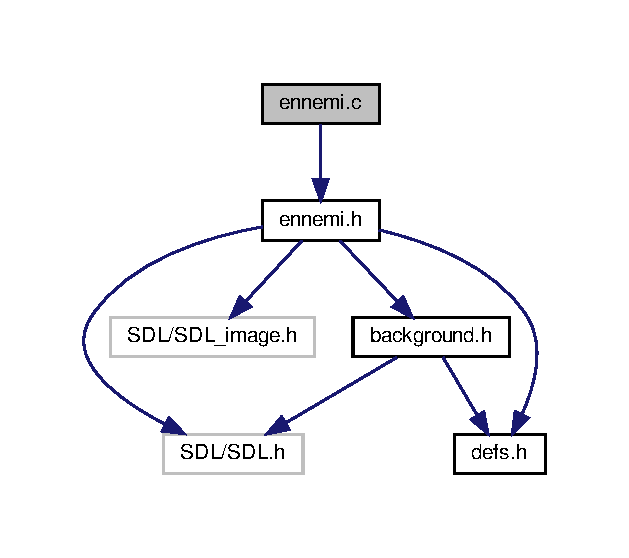
\includegraphics[width=302pt]{ennemi_8c__incl}
\end{center}
\end{figure}
\subsection*{Functions}
\begin{DoxyCompactItemize}
\item 
int \hyperlink{ennemi_8c_afde13914c19c18b1e242aa74218633e1}{init\+\_\+ennemi} (\hyperlink{structEnnemi}{Ennemi} $\ast$E, char $\ast$path)
\item 
int \hyperlink{ennemi_8c_aab02c87cdc44eb526fba24e52342a999}{load\+Ennemi\+Images} (\hyperlink{structEnnemi}{Ennemi} $\ast$A, char $\ast$path)
\item 
void \hyperlink{ennemi_8c_a33539862b507334c5b122af3ca87585c}{init\+Ennemi\+Attributes} (\hyperlink{structEnnemi}{Ennemi} $\ast$E)
\item 
void \hyperlink{ennemi_8c_a4a6d168704004408735192346353ec89}{display\+\_\+ennemi} (\hyperlink{structEnnemi}{Ennemi} E, S\+D\+L\+\_\+\+Surface $\ast$screen)
\item 
void \hyperlink{ennemi_8c_aba87f4048a9174ed4da1bfdacdb48e7a}{animate\+Ennemi} (\hyperlink{structEnnemi}{Ennemi} $\ast$E)
\item 
void \hyperlink{ennemi_8c_a6e1dcb4906c388746dde0f9319478444}{move\+Ennemi} (\hyperlink{structEnnemi}{Ennemi} $\ast$E, S\+D\+L\+\_\+\+Rect pos\+Hero)
\item 
void \hyperlink{ennemi_8c_aeb35ec28dc6bb5926a0f122f46abb838}{update\+\_\+ennemi} (\hyperlink{structEnnemi}{Ennemi} $\ast$E, S\+D\+L\+\_\+\+Rect pos\+Hero)
\item 
void \hyperlink{ennemi_8c_a94a78c5e97a5507ab163f99d68678965}{update\+Ennemi\+State} (\hyperlink{structEnnemi}{Ennemi} $\ast$E, int dist\+EH)
\item 
void \hyperlink{ennemi_8c_af0b8bd6f8504f557621c6d0c1b84bcdc}{free\+Ennemi} (\hyperlink{structEnnemi}{Ennemi} $\ast$E)
\end{DoxyCompactItemize}


\subsection{Function Documentation}
\mbox{\Hypertarget{ennemi_8c_aba87f4048a9174ed4da1bfdacdb48e7a}\label{ennemi_8c_aba87f4048a9174ed4da1bfdacdb48e7a}} 
\index{ennemi.\+c@{ennemi.\+c}!animate\+Ennemi@{animate\+Ennemi}}
\index{animate\+Ennemi@{animate\+Ennemi}!ennemi.\+c@{ennemi.\+c}}
\subsubsection{\texorpdfstring{animate\+Ennemi()}{animateEnnemi()}}
{\footnotesize\ttfamily void animate\+Ennemi (\begin{DoxyParamCaption}\item[{\hyperlink{structEnnemi}{Ennemi} $\ast$}]{E }\end{DoxyParamCaption})}

Here is the caller graph for this function\+:
\nopagebreak
\begin{figure}[H]
\begin{center}
\leavevmode
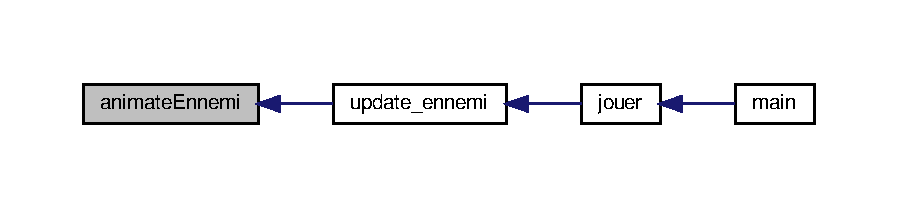
\includegraphics[width=350pt]{ennemi_8c_aba87f4048a9174ed4da1bfdacdb48e7a_icgraph}
\end{center}
\end{figure}
\mbox{\Hypertarget{ennemi_8c_a4a6d168704004408735192346353ec89}\label{ennemi_8c_a4a6d168704004408735192346353ec89}} 
\index{ennemi.\+c@{ennemi.\+c}!display\+\_\+ennemi@{display\+\_\+ennemi}}
\index{display\+\_\+ennemi@{display\+\_\+ennemi}!ennemi.\+c@{ennemi.\+c}}
\subsubsection{\texorpdfstring{display\+\_\+ennemi()}{display\_ennemi()}}
{\footnotesize\ttfamily void display\+\_\+ennemi (\begin{DoxyParamCaption}\item[{\hyperlink{structEnnemi}{Ennemi}}]{E,  }\item[{S\+D\+L\+\_\+\+Surface $\ast$}]{screen }\end{DoxyParamCaption})}

Here is the caller graph for this function\+:
\nopagebreak
\begin{figure}[H]
\begin{center}
\leavevmode
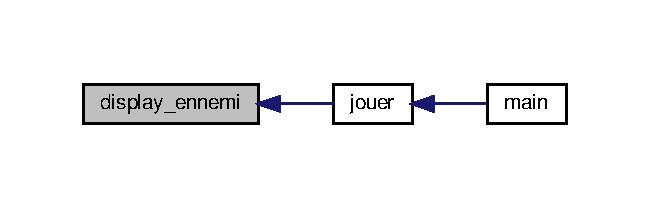
\includegraphics[width=312pt]{ennemi_8c_a4a6d168704004408735192346353ec89_icgraph}
\end{center}
\end{figure}
\mbox{\Hypertarget{ennemi_8c_af0b8bd6f8504f557621c6d0c1b84bcdc}\label{ennemi_8c_af0b8bd6f8504f557621c6d0c1b84bcdc}} 
\index{ennemi.\+c@{ennemi.\+c}!free\+Ennemi@{free\+Ennemi}}
\index{free\+Ennemi@{free\+Ennemi}!ennemi.\+c@{ennemi.\+c}}
\subsubsection{\texorpdfstring{free\+Ennemi()}{freeEnnemi()}}
{\footnotesize\ttfamily void free\+Ennemi (\begin{DoxyParamCaption}\item[{\hyperlink{structEnnemi}{Ennemi} $\ast$}]{E }\end{DoxyParamCaption})}

Here is the caller graph for this function\+:
\nopagebreak
\begin{figure}[H]
\begin{center}
\leavevmode
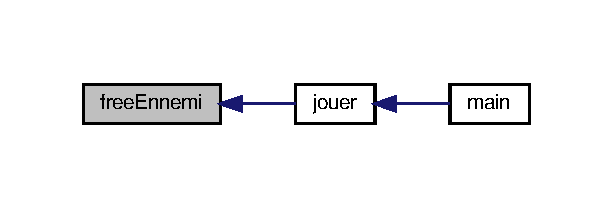
\includegraphics[width=294pt]{ennemi_8c_af0b8bd6f8504f557621c6d0c1b84bcdc_icgraph}
\end{center}
\end{figure}
\mbox{\Hypertarget{ennemi_8c_afde13914c19c18b1e242aa74218633e1}\label{ennemi_8c_afde13914c19c18b1e242aa74218633e1}} 
\index{ennemi.\+c@{ennemi.\+c}!init\+\_\+ennemi@{init\+\_\+ennemi}}
\index{init\+\_\+ennemi@{init\+\_\+ennemi}!ennemi.\+c@{ennemi.\+c}}
\subsubsection{\texorpdfstring{init\+\_\+ennemi()}{init\_ennemi()}}
{\footnotesize\ttfamily int init\+\_\+ennemi (\begin{DoxyParamCaption}\item[{\hyperlink{structEnnemi}{Ennemi} $\ast$}]{E,  }\item[{char $\ast$}]{path }\end{DoxyParamCaption})}

Here is the call graph for this function\+:
\nopagebreak
\begin{figure}[H]
\begin{center}
\leavevmode
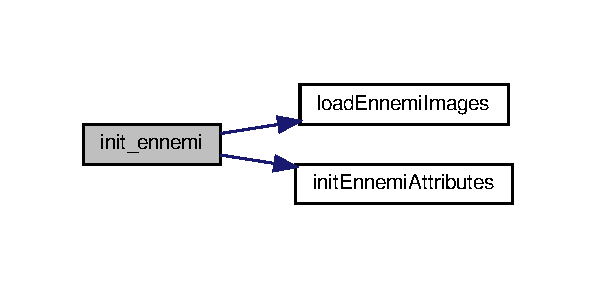
\includegraphics[width=286pt]{ennemi_8c_afde13914c19c18b1e242aa74218633e1_cgraph}
\end{center}
\end{figure}
Here is the caller graph for this function\+:
\nopagebreak
\begin{figure}[H]
\begin{center}
\leavevmode
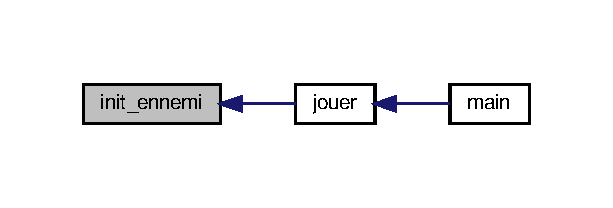
\includegraphics[width=294pt]{ennemi_8c_afde13914c19c18b1e242aa74218633e1_icgraph}
\end{center}
\end{figure}
\mbox{\Hypertarget{ennemi_8c_a33539862b507334c5b122af3ca87585c}\label{ennemi_8c_a33539862b507334c5b122af3ca87585c}} 
\index{ennemi.\+c@{ennemi.\+c}!init\+Ennemi\+Attributes@{init\+Ennemi\+Attributes}}
\index{init\+Ennemi\+Attributes@{init\+Ennemi\+Attributes}!ennemi.\+c@{ennemi.\+c}}
\subsubsection{\texorpdfstring{init\+Ennemi\+Attributes()}{initEnnemiAttributes()}}
{\footnotesize\ttfamily void init\+Ennemi\+Attributes (\begin{DoxyParamCaption}\item[{\hyperlink{structEnnemi}{Ennemi} $\ast$}]{E }\end{DoxyParamCaption})}

Here is the caller graph for this function\+:
\nopagebreak
\begin{figure}[H]
\begin{center}
\leavevmode
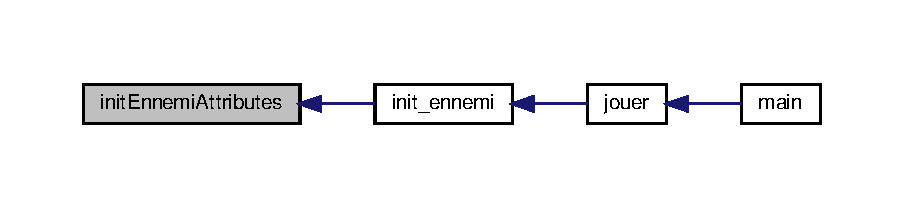
\includegraphics[width=350pt]{ennemi_8c_a33539862b507334c5b122af3ca87585c_icgraph}
\end{center}
\end{figure}
\mbox{\Hypertarget{ennemi_8c_aab02c87cdc44eb526fba24e52342a999}\label{ennemi_8c_aab02c87cdc44eb526fba24e52342a999}} 
\index{ennemi.\+c@{ennemi.\+c}!load\+Ennemi\+Images@{load\+Ennemi\+Images}}
\index{load\+Ennemi\+Images@{load\+Ennemi\+Images}!ennemi.\+c@{ennemi.\+c}}
\subsubsection{\texorpdfstring{load\+Ennemi\+Images()}{loadEnnemiImages()}}
{\footnotesize\ttfamily int load\+Ennemi\+Images (\begin{DoxyParamCaption}\item[{\hyperlink{structEnnemi}{Ennemi} $\ast$}]{A,  }\item[{char $\ast$}]{path }\end{DoxyParamCaption})}

Here is the caller graph for this function\+:
\nopagebreak
\begin{figure}[H]
\begin{center}
\leavevmode
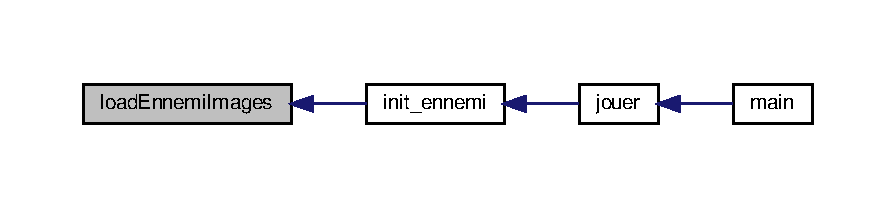
\includegraphics[width=350pt]{ennemi_8c_aab02c87cdc44eb526fba24e52342a999_icgraph}
\end{center}
\end{figure}
\mbox{\Hypertarget{ennemi_8c_a6e1dcb4906c388746dde0f9319478444}\label{ennemi_8c_a6e1dcb4906c388746dde0f9319478444}} 
\index{ennemi.\+c@{ennemi.\+c}!move\+Ennemi@{move\+Ennemi}}
\index{move\+Ennemi@{move\+Ennemi}!ennemi.\+c@{ennemi.\+c}}
\subsubsection{\texorpdfstring{move\+Ennemi()}{moveEnnemi()}}
{\footnotesize\ttfamily void move\+Ennemi (\begin{DoxyParamCaption}\item[{\hyperlink{structEnnemi}{Ennemi} $\ast$}]{E,  }\item[{S\+D\+L\+\_\+\+Rect}]{pos\+Hero }\end{DoxyParamCaption})}

Here is the caller graph for this function\+:
\nopagebreak
\begin{figure}[H]
\begin{center}
\leavevmode
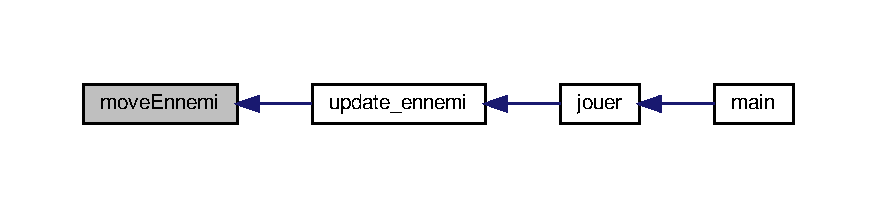
\includegraphics[width=350pt]{ennemi_8c_a6e1dcb4906c388746dde0f9319478444_icgraph}
\end{center}
\end{figure}
\mbox{\Hypertarget{ennemi_8c_aeb35ec28dc6bb5926a0f122f46abb838}\label{ennemi_8c_aeb35ec28dc6bb5926a0f122f46abb838}} 
\index{ennemi.\+c@{ennemi.\+c}!update\+\_\+ennemi@{update\+\_\+ennemi}}
\index{update\+\_\+ennemi@{update\+\_\+ennemi}!ennemi.\+c@{ennemi.\+c}}
\subsubsection{\texorpdfstring{update\+\_\+ennemi()}{update\_ennemi()}}
{\footnotesize\ttfamily void update\+\_\+ennemi (\begin{DoxyParamCaption}\item[{\hyperlink{structEnnemi}{Ennemi} $\ast$}]{E,  }\item[{S\+D\+L\+\_\+\+Rect}]{pos\+Hero }\end{DoxyParamCaption})}

Here is the call graph for this function\+:
\nopagebreak
\begin{figure}[H]
\begin{center}
\leavevmode
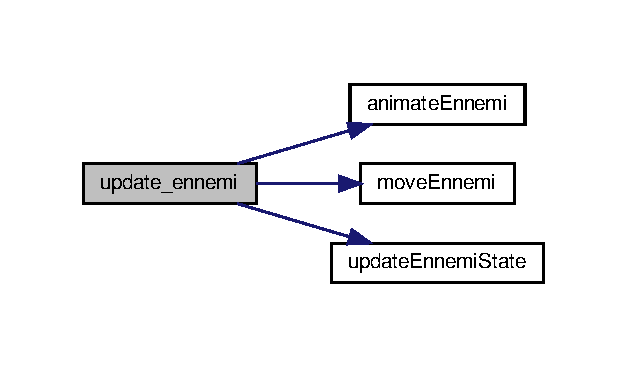
\includegraphics[width=301pt]{ennemi_8c_aeb35ec28dc6bb5926a0f122f46abb838_cgraph}
\end{center}
\end{figure}
Here is the caller graph for this function\+:
\nopagebreak
\begin{figure}[H]
\begin{center}
\leavevmode
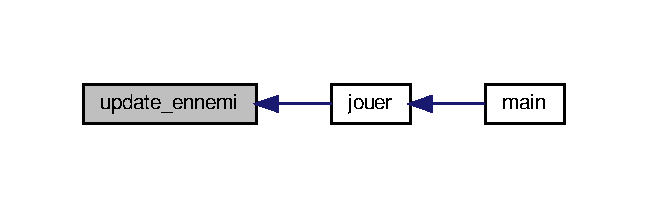
\includegraphics[width=311pt]{ennemi_8c_aeb35ec28dc6bb5926a0f122f46abb838_icgraph}
\end{center}
\end{figure}
\mbox{\Hypertarget{ennemi_8c_a94a78c5e97a5507ab163f99d68678965}\label{ennemi_8c_a94a78c5e97a5507ab163f99d68678965}} 
\index{ennemi.\+c@{ennemi.\+c}!update\+Ennemi\+State@{update\+Ennemi\+State}}
\index{update\+Ennemi\+State@{update\+Ennemi\+State}!ennemi.\+c@{ennemi.\+c}}
\subsubsection{\texorpdfstring{update\+Ennemi\+State()}{updateEnnemiState()}}
{\footnotesize\ttfamily void update\+Ennemi\+State (\begin{DoxyParamCaption}\item[{\hyperlink{structEnnemi}{Ennemi} $\ast$}]{E,  }\item[{int}]{dist\+EH }\end{DoxyParamCaption})}

Here is the caller graph for this function\+:
\nopagebreak
\begin{figure}[H]
\begin{center}
\leavevmode
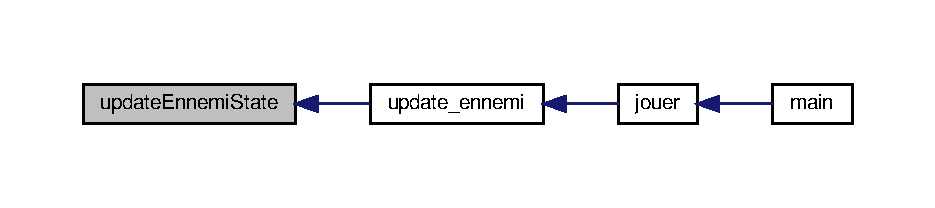
\includegraphics[width=350pt]{ennemi_8c_a94a78c5e97a5507ab163f99d68678965_icgraph}
\end{center}
\end{figure}

\hypertarget{ennemi_8h}{}\section{ennemi.\+h File Reference}
\label{ennemi_8h}\index{ennemi.\+h@{ennemi.\+h}}
{\ttfamily \#include $<$S\+D\+L/\+S\+D\+L.\+h$>$}\newline
{\ttfamily \#include $<$S\+D\+L/\+S\+D\+L\+\_\+image.\+h$>$}\newline
{\ttfamily \#include \char`\"{}defs.\+h\char`\"{}}\newline
{\ttfamily \#include \char`\"{}background.\+h\char`\"{}}\newline
Include dependency graph for ennemi.\+h\+:
\nopagebreak
\begin{figure}[H]
\begin{center}
\leavevmode
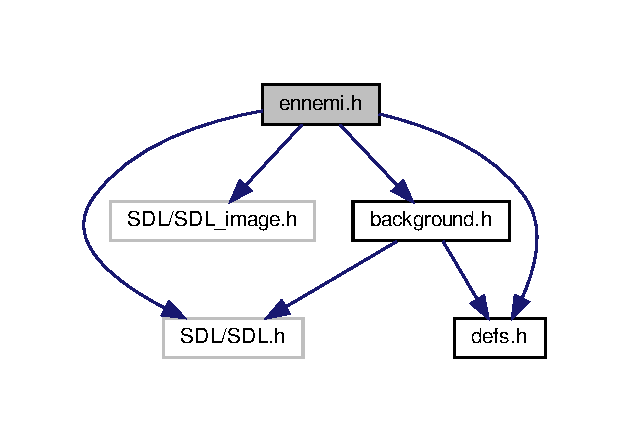
\includegraphics[width=302pt]{ennemi_8h__incl}
\end{center}
\end{figure}
This graph shows which files directly or indirectly include this file\+:
\nopagebreak
\begin{figure}[H]
\begin{center}
\leavevmode
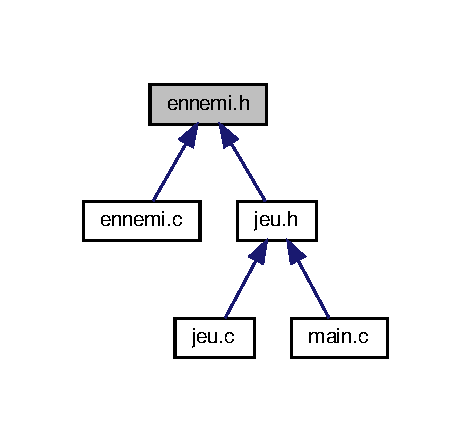
\includegraphics[width=226pt]{ennemi_8h__dep__incl}
\end{center}
\end{figure}
\subsection*{Classes}
\begin{DoxyCompactItemize}
\item 
struct \hyperlink{structEnnemi}{Ennemi}
\end{DoxyCompactItemize}
\subsection*{Typedefs}
\begin{DoxyCompactItemize}
\item 
typedef enum \hyperlink{ennemi_8h_a275a67132f10277ada3a0ee3d616b647}{S\+T\+A\+TE} \hyperlink{ennemi_8h_a6fc73911e78d07bcceea8f8ed0d87f97}{S\+T\+A\+TE}
\item 
typedef struct \hyperlink{structEnnemi}{Ennemi} \hyperlink{ennemi_8h_a768e2f7a7c4af3aa5796682238d4473b}{Ennemi}
\end{DoxyCompactItemize}
\subsection*{Enumerations}
\begin{DoxyCompactItemize}
\item 
enum \hyperlink{ennemi_8h_a275a67132f10277ada3a0ee3d616b647}{S\+T\+A\+TE} \{ \newline
\hyperlink{ennemi_8h_a275a67132f10277ada3a0ee3d616b647a757971c0bc5a1972d5f1b1be2c0e2087}{W\+A\+I\+T\+I\+NG}, 
\hyperlink{ennemi_8h_a275a67132f10277ada3a0ee3d616b647ac241aecbe2e3eba2f42ce28777f6ab65}{F\+O\+L\+L\+O\+W\+I\+NG}, 
\hyperlink{ennemi_8h_a275a67132f10277ada3a0ee3d616b647a05f520974a8946a4b11907b698557a8b}{A\+T\+T\+A\+C\+K\+I\+NG}, 
\hyperlink{ennemi_8h_a275a67132f10277ada3a0ee3d616b647a1061be6c3fb88d32829cba6f6b2be304}{R\+U\+N\+N\+I\+NG}, 
\newline
\hyperlink{ennemi_8h_a275a67132f10277ada3a0ee3d616b647a16ebdcb23eb5337fd5bc598fa8d6035d}{M\+O\+V\+I\+NG}, 
\hyperlink{ennemi_8h_a275a67132f10277ada3a0ee3d616b647acad9497b864311f7f80cf6c1a39cff1e}{M\+O\+V\+I\+N\+G1}
 \}
\end{DoxyCompactItemize}
\subsection*{Functions}
\begin{DoxyCompactItemize}
\item 
int \hyperlink{ennemi_8h_afde13914c19c18b1e242aa74218633e1}{init\+\_\+ennemi} (\hyperlink{structEnnemi}{Ennemi} $\ast$E, char $\ast$path)
\item 
void \hyperlink{ennemi_8h_aeb35ec28dc6bb5926a0f122f46abb838}{update\+\_\+ennemi} (\hyperlink{structEnnemi}{Ennemi} $\ast$E, S\+D\+L\+\_\+\+Rect pos\+Hero)
\item 
void \hyperlink{ennemi_8h_a4a6d168704004408735192346353ec89}{display\+\_\+ennemi} (\hyperlink{structEnnemi}{Ennemi} E, S\+D\+L\+\_\+\+Surface $\ast$screen)
\item 
void \hyperlink{ennemi_8h_af0b8bd6f8504f557621c6d0c1b84bcdc}{free\+Ennemi} (\hyperlink{structEnnemi}{Ennemi} $\ast$E)
\item 
int \hyperlink{ennemi_8h_a890cc605798f8bf561edf396fd041d86}{load\+Ennemi\+Images} (\hyperlink{structEnnemi}{Ennemi} $\ast$E, char $\ast$path)
\item 
void \hyperlink{ennemi_8h_a33539862b507334c5b122af3ca87585c}{init\+Ennemi\+Attributes} (\hyperlink{structEnnemi}{Ennemi} $\ast$E)
\item 
void \hyperlink{ennemi_8h_a30120a1bc5f558fc824c5fd138591101}{anim} (\hyperlink{structEnnemi}{Ennemi} $\ast$E)
\item 
void \hyperlink{ennemi_8h_a3d1e679dc09af35d772f6a5c0940827d}{anim2} (\hyperlink{structEnnemi}{Ennemi} $\ast$E)
\item 
void \hyperlink{ennemi_8h_aba87f4048a9174ed4da1bfdacdb48e7a}{animate\+Ennemi} (\hyperlink{structEnnemi}{Ennemi} $\ast$E)
\item 
void \hyperlink{ennemi_8h_a6e1dcb4906c388746dde0f9319478444}{move\+Ennemi} (\hyperlink{structEnnemi}{Ennemi} $\ast$E, S\+D\+L\+\_\+\+Rect pos\+Hero)
\item 
void \hyperlink{ennemi_8h_a2296e3eed70f4b2af8e4410af1bb9515}{move\+Ennemi2} (\hyperlink{structEnnemi}{Ennemi} $\ast$E, S\+D\+L\+\_\+\+Rect pos\+Hero)
\item 
void \hyperlink{ennemi_8h_ad7ec9344783c062b86c69da4d2a2632f}{move\+Ennemi3} (\hyperlink{structEnnemi}{Ennemi} $\ast$E, S\+D\+L\+\_\+\+Rect pos\+Hero)
\item 
void \hyperlink{ennemi_8h_a94a78c5e97a5507ab163f99d68678965}{update\+Ennemi\+State} (\hyperlink{structEnnemi}{Ennemi} $\ast$E, int dist\+EH)
\end{DoxyCompactItemize}


\subsection{Typedef Documentation}
\mbox{\Hypertarget{ennemi_8h_a768e2f7a7c4af3aa5796682238d4473b}\label{ennemi_8h_a768e2f7a7c4af3aa5796682238d4473b}} 
\index{ennemi.\+h@{ennemi.\+h}!Ennemi@{Ennemi}}
\index{Ennemi@{Ennemi}!ennemi.\+h@{ennemi.\+h}}
\subsubsection{\texorpdfstring{Ennemi}{Ennemi}}
{\footnotesize\ttfamily typedef struct \hyperlink{structEnnemi}{Ennemi} \hyperlink{structEnnemi}{Ennemi}}

\mbox{\Hypertarget{ennemi_8h_a6fc73911e78d07bcceea8f8ed0d87f97}\label{ennemi_8h_a6fc73911e78d07bcceea8f8ed0d87f97}} 
\index{ennemi.\+h@{ennemi.\+h}!S\+T\+A\+TE@{S\+T\+A\+TE}}
\index{S\+T\+A\+TE@{S\+T\+A\+TE}!ennemi.\+h@{ennemi.\+h}}
\subsubsection{\texorpdfstring{S\+T\+A\+TE}{STATE}}
{\footnotesize\ttfamily typedef enum \hyperlink{ennemi_8h_a275a67132f10277ada3a0ee3d616b647}{S\+T\+A\+TE} \hyperlink{ennemi_8h_a275a67132f10277ada3a0ee3d616b647}{S\+T\+A\+TE}}



\subsection{Enumeration Type Documentation}
\mbox{\Hypertarget{ennemi_8h_a275a67132f10277ada3a0ee3d616b647}\label{ennemi_8h_a275a67132f10277ada3a0ee3d616b647}} 
\index{ennemi.\+h@{ennemi.\+h}!S\+T\+A\+TE@{S\+T\+A\+TE}}
\index{S\+T\+A\+TE@{S\+T\+A\+TE}!ennemi.\+h@{ennemi.\+h}}
\subsubsection{\texorpdfstring{S\+T\+A\+TE}{STATE}}
{\footnotesize\ttfamily enum \hyperlink{ennemi_8h_a275a67132f10277ada3a0ee3d616b647}{S\+T\+A\+TE}}

\begin{DoxyEnumFields}{Enumerator}
\raisebox{\heightof{T}}[0pt][0pt]{\index{W\+A\+I\+T\+I\+NG@{W\+A\+I\+T\+I\+NG}!ennemi.\+h@{ennemi.\+h}}\index{ennemi.\+h@{ennemi.\+h}!W\+A\+I\+T\+I\+NG@{W\+A\+I\+T\+I\+NG}}}\mbox{\Hypertarget{ennemi_8h_a275a67132f10277ada3a0ee3d616b647a757971c0bc5a1972d5f1b1be2c0e2087}\label{ennemi_8h_a275a67132f10277ada3a0ee3d616b647a757971c0bc5a1972d5f1b1be2c0e2087}} 
W\+A\+I\+T\+I\+NG&\\
\hline

\raisebox{\heightof{T}}[0pt][0pt]{\index{F\+O\+L\+L\+O\+W\+I\+NG@{F\+O\+L\+L\+O\+W\+I\+NG}!ennemi.\+h@{ennemi.\+h}}\index{ennemi.\+h@{ennemi.\+h}!F\+O\+L\+L\+O\+W\+I\+NG@{F\+O\+L\+L\+O\+W\+I\+NG}}}\mbox{\Hypertarget{ennemi_8h_a275a67132f10277ada3a0ee3d616b647ac241aecbe2e3eba2f42ce28777f6ab65}\label{ennemi_8h_a275a67132f10277ada3a0ee3d616b647ac241aecbe2e3eba2f42ce28777f6ab65}} 
F\+O\+L\+L\+O\+W\+I\+NG&\\
\hline

\raisebox{\heightof{T}}[0pt][0pt]{\index{A\+T\+T\+A\+C\+K\+I\+NG@{A\+T\+T\+A\+C\+K\+I\+NG}!ennemi.\+h@{ennemi.\+h}}\index{ennemi.\+h@{ennemi.\+h}!A\+T\+T\+A\+C\+K\+I\+NG@{A\+T\+T\+A\+C\+K\+I\+NG}}}\mbox{\Hypertarget{ennemi_8h_a275a67132f10277ada3a0ee3d616b647a05f520974a8946a4b11907b698557a8b}\label{ennemi_8h_a275a67132f10277ada3a0ee3d616b647a05f520974a8946a4b11907b698557a8b}} 
A\+T\+T\+A\+C\+K\+I\+NG&\\
\hline

\raisebox{\heightof{T}}[0pt][0pt]{\index{R\+U\+N\+N\+I\+NG@{R\+U\+N\+N\+I\+NG}!ennemi.\+h@{ennemi.\+h}}\index{ennemi.\+h@{ennemi.\+h}!R\+U\+N\+N\+I\+NG@{R\+U\+N\+N\+I\+NG}}}\mbox{\Hypertarget{ennemi_8h_a275a67132f10277ada3a0ee3d616b647a1061be6c3fb88d32829cba6f6b2be304}\label{ennemi_8h_a275a67132f10277ada3a0ee3d616b647a1061be6c3fb88d32829cba6f6b2be304}} 
R\+U\+N\+N\+I\+NG&\\
\hline

\raisebox{\heightof{T}}[0pt][0pt]{\index{M\+O\+V\+I\+NG@{M\+O\+V\+I\+NG}!ennemi.\+h@{ennemi.\+h}}\index{ennemi.\+h@{ennemi.\+h}!M\+O\+V\+I\+NG@{M\+O\+V\+I\+NG}}}\mbox{\Hypertarget{ennemi_8h_a275a67132f10277ada3a0ee3d616b647a16ebdcb23eb5337fd5bc598fa8d6035d}\label{ennemi_8h_a275a67132f10277ada3a0ee3d616b647a16ebdcb23eb5337fd5bc598fa8d6035d}} 
M\+O\+V\+I\+NG&\\
\hline

\raisebox{\heightof{T}}[0pt][0pt]{\index{M\+O\+V\+I\+N\+G1@{M\+O\+V\+I\+N\+G1}!ennemi.\+h@{ennemi.\+h}}\index{ennemi.\+h@{ennemi.\+h}!M\+O\+V\+I\+N\+G1@{M\+O\+V\+I\+N\+G1}}}\mbox{\Hypertarget{ennemi_8h_a275a67132f10277ada3a0ee3d616b647acad9497b864311f7f80cf6c1a39cff1e}\label{ennemi_8h_a275a67132f10277ada3a0ee3d616b647acad9497b864311f7f80cf6c1a39cff1e}} 
M\+O\+V\+I\+N\+G1&\\
\hline

\end{DoxyEnumFields}


\subsection{Function Documentation}
\mbox{\Hypertarget{ennemi_8h_a30120a1bc5f558fc824c5fd138591101}\label{ennemi_8h_a30120a1bc5f558fc824c5fd138591101}} 
\index{ennemi.\+h@{ennemi.\+h}!anim@{anim}}
\index{anim@{anim}!ennemi.\+h@{ennemi.\+h}}
\subsubsection{\texorpdfstring{anim()}{anim()}}
{\footnotesize\ttfamily void anim (\begin{DoxyParamCaption}\item[{\hyperlink{structEnnemi}{Ennemi} $\ast$}]{E }\end{DoxyParamCaption})}

\mbox{\Hypertarget{ennemi_8h_a3d1e679dc09af35d772f6a5c0940827d}\label{ennemi_8h_a3d1e679dc09af35d772f6a5c0940827d}} 
\index{ennemi.\+h@{ennemi.\+h}!anim2@{anim2}}
\index{anim2@{anim2}!ennemi.\+h@{ennemi.\+h}}
\subsubsection{\texorpdfstring{anim2()}{anim2()}}
{\footnotesize\ttfamily void anim2 (\begin{DoxyParamCaption}\item[{\hyperlink{structEnnemi}{Ennemi} $\ast$}]{E }\end{DoxyParamCaption})}

\mbox{\Hypertarget{ennemi_8h_aba87f4048a9174ed4da1bfdacdb48e7a}\label{ennemi_8h_aba87f4048a9174ed4da1bfdacdb48e7a}} 
\index{ennemi.\+h@{ennemi.\+h}!animate\+Ennemi@{animate\+Ennemi}}
\index{animate\+Ennemi@{animate\+Ennemi}!ennemi.\+h@{ennemi.\+h}}
\subsubsection{\texorpdfstring{animate\+Ennemi()}{animateEnnemi()}}
{\footnotesize\ttfamily void animate\+Ennemi (\begin{DoxyParamCaption}\item[{\hyperlink{structEnnemi}{Ennemi} $\ast$}]{E }\end{DoxyParamCaption})}

Here is the caller graph for this function\+:
\nopagebreak
\begin{figure}[H]
\begin{center}
\leavevmode
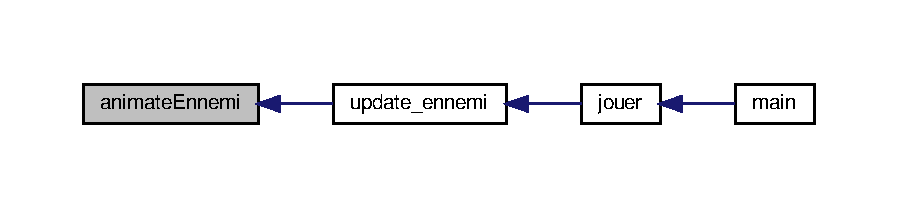
\includegraphics[width=350pt]{ennemi_8h_aba87f4048a9174ed4da1bfdacdb48e7a_icgraph}
\end{center}
\end{figure}
\mbox{\Hypertarget{ennemi_8h_a4a6d168704004408735192346353ec89}\label{ennemi_8h_a4a6d168704004408735192346353ec89}} 
\index{ennemi.\+h@{ennemi.\+h}!display\+\_\+ennemi@{display\+\_\+ennemi}}
\index{display\+\_\+ennemi@{display\+\_\+ennemi}!ennemi.\+h@{ennemi.\+h}}
\subsubsection{\texorpdfstring{display\+\_\+ennemi()}{display\_ennemi()}}
{\footnotesize\ttfamily void display\+\_\+ennemi (\begin{DoxyParamCaption}\item[{\hyperlink{structEnnemi}{Ennemi}}]{E,  }\item[{S\+D\+L\+\_\+\+Surface $\ast$}]{screen }\end{DoxyParamCaption})}

Here is the caller graph for this function\+:
\nopagebreak
\begin{figure}[H]
\begin{center}
\leavevmode
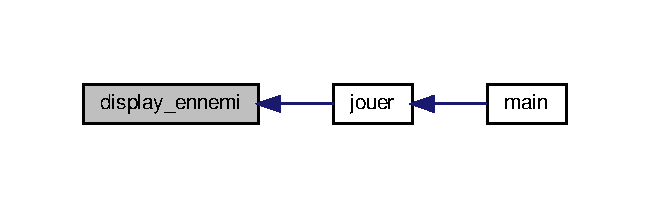
\includegraphics[width=312pt]{ennemi_8h_a4a6d168704004408735192346353ec89_icgraph}
\end{center}
\end{figure}
\mbox{\Hypertarget{ennemi_8h_af0b8bd6f8504f557621c6d0c1b84bcdc}\label{ennemi_8h_af0b8bd6f8504f557621c6d0c1b84bcdc}} 
\index{ennemi.\+h@{ennemi.\+h}!free\+Ennemi@{free\+Ennemi}}
\index{free\+Ennemi@{free\+Ennemi}!ennemi.\+h@{ennemi.\+h}}
\subsubsection{\texorpdfstring{free\+Ennemi()}{freeEnnemi()}}
{\footnotesize\ttfamily void free\+Ennemi (\begin{DoxyParamCaption}\item[{\hyperlink{structEnnemi}{Ennemi} $\ast$}]{E }\end{DoxyParamCaption})}

Here is the caller graph for this function\+:
\nopagebreak
\begin{figure}[H]
\begin{center}
\leavevmode
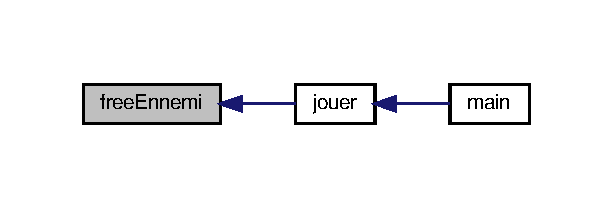
\includegraphics[width=294pt]{ennemi_8h_af0b8bd6f8504f557621c6d0c1b84bcdc_icgraph}
\end{center}
\end{figure}
\mbox{\Hypertarget{ennemi_8h_afde13914c19c18b1e242aa74218633e1}\label{ennemi_8h_afde13914c19c18b1e242aa74218633e1}} 
\index{ennemi.\+h@{ennemi.\+h}!init\+\_\+ennemi@{init\+\_\+ennemi}}
\index{init\+\_\+ennemi@{init\+\_\+ennemi}!ennemi.\+h@{ennemi.\+h}}
\subsubsection{\texorpdfstring{init\+\_\+ennemi()}{init\_ennemi()}}
{\footnotesize\ttfamily int init\+\_\+ennemi (\begin{DoxyParamCaption}\item[{\hyperlink{structEnnemi}{Ennemi} $\ast$}]{E,  }\item[{char $\ast$}]{path }\end{DoxyParamCaption})}

Here is the call graph for this function\+:
\nopagebreak
\begin{figure}[H]
\begin{center}
\leavevmode
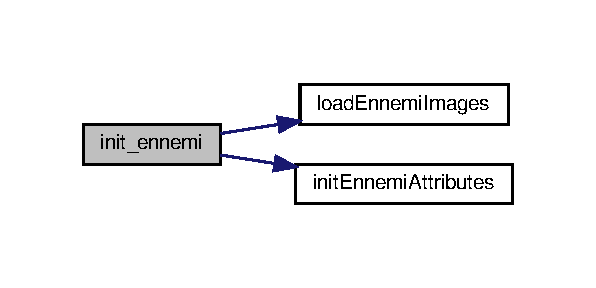
\includegraphics[width=286pt]{ennemi_8h_afde13914c19c18b1e242aa74218633e1_cgraph}
\end{center}
\end{figure}
Here is the caller graph for this function\+:
\nopagebreak
\begin{figure}[H]
\begin{center}
\leavevmode
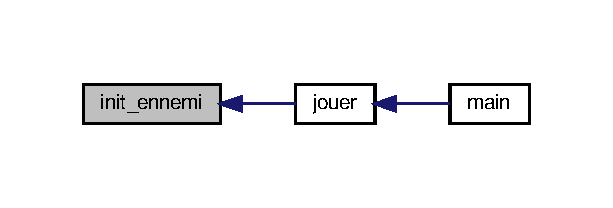
\includegraphics[width=294pt]{ennemi_8h_afde13914c19c18b1e242aa74218633e1_icgraph}
\end{center}
\end{figure}
\mbox{\Hypertarget{ennemi_8h_a33539862b507334c5b122af3ca87585c}\label{ennemi_8h_a33539862b507334c5b122af3ca87585c}} 
\index{ennemi.\+h@{ennemi.\+h}!init\+Ennemi\+Attributes@{init\+Ennemi\+Attributes}}
\index{init\+Ennemi\+Attributes@{init\+Ennemi\+Attributes}!ennemi.\+h@{ennemi.\+h}}
\subsubsection{\texorpdfstring{init\+Ennemi\+Attributes()}{initEnnemiAttributes()}}
{\footnotesize\ttfamily void init\+Ennemi\+Attributes (\begin{DoxyParamCaption}\item[{\hyperlink{structEnnemi}{Ennemi} $\ast$}]{E }\end{DoxyParamCaption})}

Here is the caller graph for this function\+:
\nopagebreak
\begin{figure}[H]
\begin{center}
\leavevmode
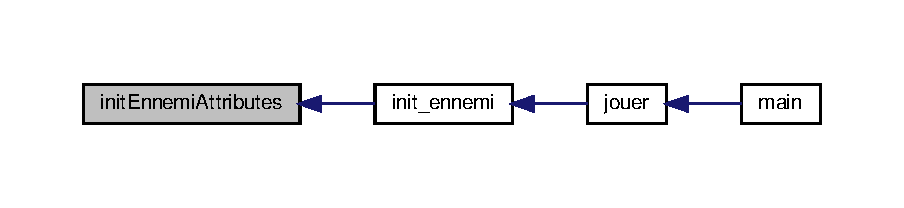
\includegraphics[width=350pt]{ennemi_8h_a33539862b507334c5b122af3ca87585c_icgraph}
\end{center}
\end{figure}
\mbox{\Hypertarget{ennemi_8h_a890cc605798f8bf561edf396fd041d86}\label{ennemi_8h_a890cc605798f8bf561edf396fd041d86}} 
\index{ennemi.\+h@{ennemi.\+h}!load\+Ennemi\+Images@{load\+Ennemi\+Images}}
\index{load\+Ennemi\+Images@{load\+Ennemi\+Images}!ennemi.\+h@{ennemi.\+h}}
\subsubsection{\texorpdfstring{load\+Ennemi\+Images()}{loadEnnemiImages()}}
{\footnotesize\ttfamily int load\+Ennemi\+Images (\begin{DoxyParamCaption}\item[{\hyperlink{structEnnemi}{Ennemi} $\ast$}]{E,  }\item[{char $\ast$}]{path }\end{DoxyParamCaption})}

Here is the caller graph for this function\+:
\nopagebreak
\begin{figure}[H]
\begin{center}
\leavevmode
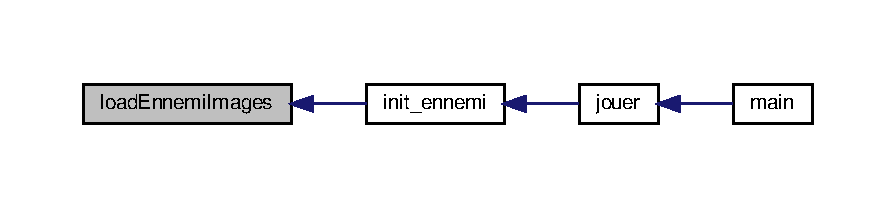
\includegraphics[width=350pt]{ennemi_8h_a890cc605798f8bf561edf396fd041d86_icgraph}
\end{center}
\end{figure}
\mbox{\Hypertarget{ennemi_8h_a6e1dcb4906c388746dde0f9319478444}\label{ennemi_8h_a6e1dcb4906c388746dde0f9319478444}} 
\index{ennemi.\+h@{ennemi.\+h}!move\+Ennemi@{move\+Ennemi}}
\index{move\+Ennemi@{move\+Ennemi}!ennemi.\+h@{ennemi.\+h}}
\subsubsection{\texorpdfstring{move\+Ennemi()}{moveEnnemi()}}
{\footnotesize\ttfamily void move\+Ennemi (\begin{DoxyParamCaption}\item[{\hyperlink{structEnnemi}{Ennemi} $\ast$}]{E,  }\item[{S\+D\+L\+\_\+\+Rect}]{pos\+Hero }\end{DoxyParamCaption})}

Here is the caller graph for this function\+:
\nopagebreak
\begin{figure}[H]
\begin{center}
\leavevmode
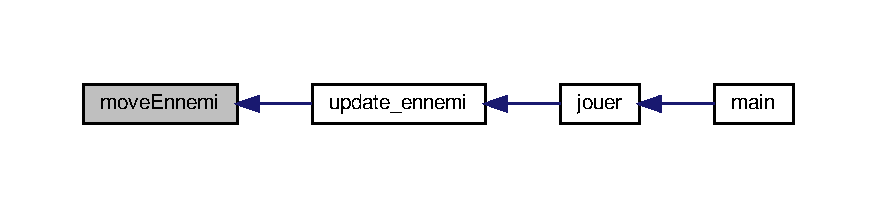
\includegraphics[width=350pt]{ennemi_8h_a6e1dcb4906c388746dde0f9319478444_icgraph}
\end{center}
\end{figure}
\mbox{\Hypertarget{ennemi_8h_a2296e3eed70f4b2af8e4410af1bb9515}\label{ennemi_8h_a2296e3eed70f4b2af8e4410af1bb9515}} 
\index{ennemi.\+h@{ennemi.\+h}!move\+Ennemi2@{move\+Ennemi2}}
\index{move\+Ennemi2@{move\+Ennemi2}!ennemi.\+h@{ennemi.\+h}}
\subsubsection{\texorpdfstring{move\+Ennemi2()}{moveEnnemi2()}}
{\footnotesize\ttfamily void move\+Ennemi2 (\begin{DoxyParamCaption}\item[{\hyperlink{structEnnemi}{Ennemi} $\ast$}]{E,  }\item[{S\+D\+L\+\_\+\+Rect}]{pos\+Hero }\end{DoxyParamCaption})}

\mbox{\Hypertarget{ennemi_8h_ad7ec9344783c062b86c69da4d2a2632f}\label{ennemi_8h_ad7ec9344783c062b86c69da4d2a2632f}} 
\index{ennemi.\+h@{ennemi.\+h}!move\+Ennemi3@{move\+Ennemi3}}
\index{move\+Ennemi3@{move\+Ennemi3}!ennemi.\+h@{ennemi.\+h}}
\subsubsection{\texorpdfstring{move\+Ennemi3()}{moveEnnemi3()}}
{\footnotesize\ttfamily void move\+Ennemi3 (\begin{DoxyParamCaption}\item[{\hyperlink{structEnnemi}{Ennemi} $\ast$}]{E,  }\item[{S\+D\+L\+\_\+\+Rect}]{pos\+Hero }\end{DoxyParamCaption})}

\mbox{\Hypertarget{ennemi_8h_aeb35ec28dc6bb5926a0f122f46abb838}\label{ennemi_8h_aeb35ec28dc6bb5926a0f122f46abb838}} 
\index{ennemi.\+h@{ennemi.\+h}!update\+\_\+ennemi@{update\+\_\+ennemi}}
\index{update\+\_\+ennemi@{update\+\_\+ennemi}!ennemi.\+h@{ennemi.\+h}}
\subsubsection{\texorpdfstring{update\+\_\+ennemi()}{update\_ennemi()}}
{\footnotesize\ttfamily void update\+\_\+ennemi (\begin{DoxyParamCaption}\item[{\hyperlink{structEnnemi}{Ennemi} $\ast$}]{E,  }\item[{S\+D\+L\+\_\+\+Rect}]{pos\+Hero }\end{DoxyParamCaption})}

Here is the call graph for this function\+:
\nopagebreak
\begin{figure}[H]
\begin{center}
\leavevmode
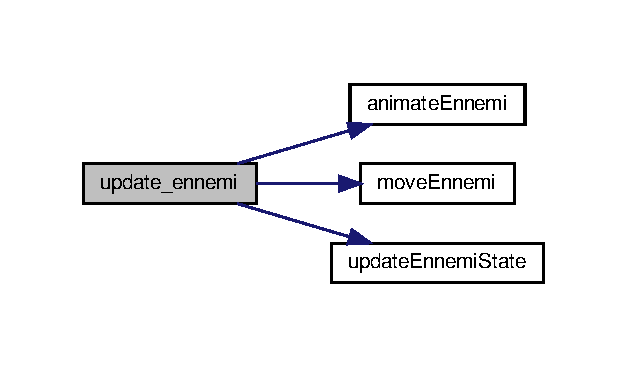
\includegraphics[width=301pt]{ennemi_8h_aeb35ec28dc6bb5926a0f122f46abb838_cgraph}
\end{center}
\end{figure}
Here is the caller graph for this function\+:
\nopagebreak
\begin{figure}[H]
\begin{center}
\leavevmode
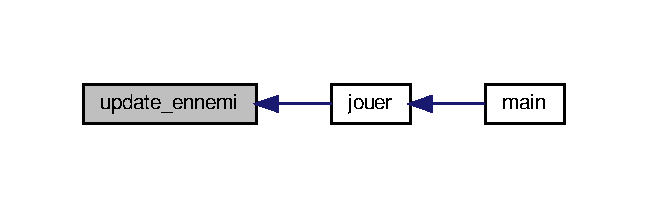
\includegraphics[width=311pt]{ennemi_8h_aeb35ec28dc6bb5926a0f122f46abb838_icgraph}
\end{center}
\end{figure}
\mbox{\Hypertarget{ennemi_8h_a94a78c5e97a5507ab163f99d68678965}\label{ennemi_8h_a94a78c5e97a5507ab163f99d68678965}} 
\index{ennemi.\+h@{ennemi.\+h}!update\+Ennemi\+State@{update\+Ennemi\+State}}
\index{update\+Ennemi\+State@{update\+Ennemi\+State}!ennemi.\+h@{ennemi.\+h}}
\subsubsection{\texorpdfstring{update\+Ennemi\+State()}{updateEnnemiState()}}
{\footnotesize\ttfamily void update\+Ennemi\+State (\begin{DoxyParamCaption}\item[{\hyperlink{structEnnemi}{Ennemi} $\ast$}]{E,  }\item[{int}]{dist\+EH }\end{DoxyParamCaption})}

Here is the caller graph for this function\+:
\nopagebreak
\begin{figure}[H]
\begin{center}
\leavevmode
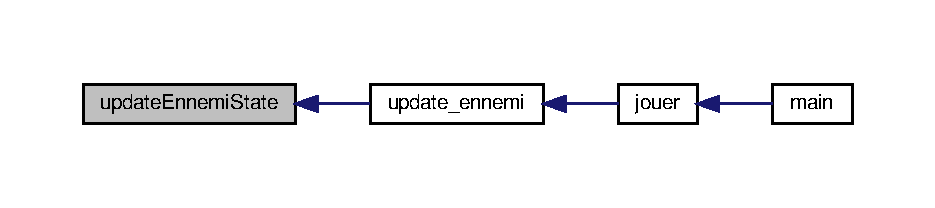
\includegraphics[width=350pt]{ennemi_8h_a94a78c5e97a5507ab163f99d68678965_icgraph}
\end{center}
\end{figure}

\hypertarget{hero_8c}{}\section{hero.\+c File Reference}
\label{hero_8c}\index{hero.\+c@{hero.\+c}}
{\ttfamily \#include \char`\"{}hero.\+h\char`\"{}}\newline
Include dependency graph for hero.\+c\+:
\nopagebreak
\begin{figure}[H]
\begin{center}
\leavevmode
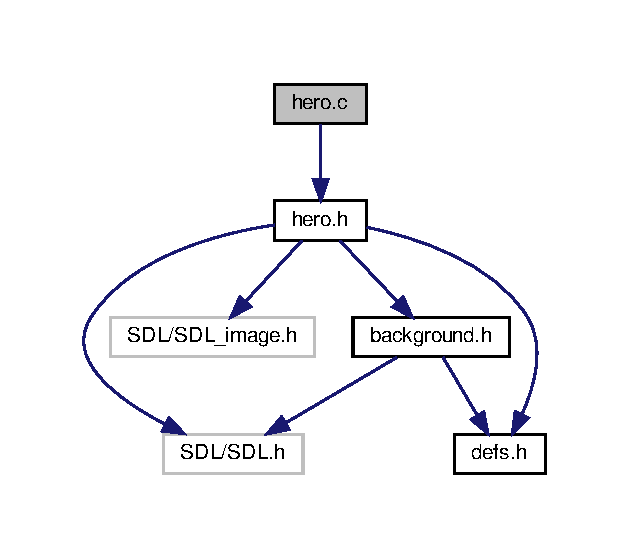
\includegraphics[width=302pt]{hero_8c__incl}
\end{center}
\end{figure}
\subsection*{Functions}
\begin{DoxyCompactItemize}
\item 
int \hyperlink{hero_8c_a02de6fcfc96882d79393b481b079c8d3}{init\+\_\+hero} (\hyperlink{hero_8h_aea2a78936086ab032e9479a22f656a5a}{Hero} $\ast$H, char $\ast$path)
\item 
int \hyperlink{hero_8c_ae11170e307c1823f644a0ed6c4fcb3d3}{load\+Hero\+Images} (\hyperlink{hero_8h_aea2a78936086ab032e9479a22f656a5a}{Hero} $\ast$H, char $\ast$path)
\item 
void \hyperlink{hero_8c_afb70c3dc1353ca52fb962b1b5e341257}{init\+Hero\+Attributes} (\hyperlink{hero_8h_aea2a78936086ab032e9479a22f656a5a}{Hero} $\ast$H)
\item 
void \hyperlink{hero_8c_a5ed7845fc23601c05b518e32b72edc45}{display\+\_\+hero} (\hyperlink{hero_8h_aea2a78936086ab032e9479a22f656a5a}{Hero} H, S\+D\+L\+\_\+\+Surface $\ast$screen)
\item 
void \hyperlink{hero_8c_a8d9990c46b5900c912fc96d4b091999f}{update\+\_\+hero} (\hyperlink{hero_8h_aea2a78936086ab032e9479a22f656a5a}{Hero} $\ast$H, int Tab\+\_\+input\mbox{[}$\,$\mbox{]}, int H\+E\+\_\+collision)
\item 
void \hyperlink{hero_8c_a19b2ddbd3df2e9dd40de2dd5b5f33d37}{animate\+Hero} (\hyperlink{hero_8h_aea2a78936086ab032e9479a22f656a5a}{Hero} $\ast$H, int Tab\+\_\+input\mbox{[}$\,$\mbox{]}, int H\+E\+\_\+collision)
\item 
void \hyperlink{hero_8c_a949611862d28f49bddbb4db1bf587ebe}{move\+Hero} (\hyperlink{hero_8h_aea2a78936086ab032e9479a22f656a5a}{Hero} $\ast$H, int Tab\+\_\+input\mbox{[}$\,$\mbox{]})
\item 
void \hyperlink{hero_8c_a219651f087e4676983a70d84e7f79f13}{update\+Hero\+Score} (\hyperlink{hero_8h_aea2a78936086ab032e9479a22f656a5a}{Hero} $\ast$H, int H\+E\+\_\+collision)
\item 
void \hyperlink{hero_8c_a72d8438912e0fab3e100d52b2560845e}{free\+Hero} (\hyperlink{hero_8h_aea2a78936086ab032e9479a22f656a5a}{Hero} $\ast$H)
\end{DoxyCompactItemize}


\subsection{Function Documentation}
\mbox{\Hypertarget{hero_8c_a19b2ddbd3df2e9dd40de2dd5b5f33d37}\label{hero_8c_a19b2ddbd3df2e9dd40de2dd5b5f33d37}} 
\index{hero.\+c@{hero.\+c}!animate\+Hero@{animate\+Hero}}
\index{animate\+Hero@{animate\+Hero}!hero.\+c@{hero.\+c}}
\subsubsection{\texorpdfstring{animate\+Hero()}{animateHero()}}
{\footnotesize\ttfamily void animate\+Hero (\begin{DoxyParamCaption}\item[{\hyperlink{hero_8h_aea2a78936086ab032e9479a22f656a5a}{Hero} $\ast$}]{H,  }\item[{int}]{Tab\+\_\+input\mbox{[}$\,$\mbox{]},  }\item[{int}]{H\+E\+\_\+collision }\end{DoxyParamCaption})}

Here is the caller graph for this function\+:
\nopagebreak
\begin{figure}[H]
\begin{center}
\leavevmode
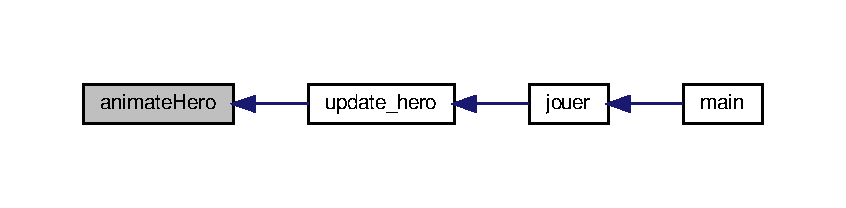
\includegraphics[width=350pt]{hero_8c_a19b2ddbd3df2e9dd40de2dd5b5f33d37_icgraph}
\end{center}
\end{figure}
\mbox{\Hypertarget{hero_8c_a5ed7845fc23601c05b518e32b72edc45}\label{hero_8c_a5ed7845fc23601c05b518e32b72edc45}} 
\index{hero.\+c@{hero.\+c}!display\+\_\+hero@{display\+\_\+hero}}
\index{display\+\_\+hero@{display\+\_\+hero}!hero.\+c@{hero.\+c}}
\subsubsection{\texorpdfstring{display\+\_\+hero()}{display\_hero()}}
{\footnotesize\ttfamily void display\+\_\+hero (\begin{DoxyParamCaption}\item[{\hyperlink{hero_8h_aea2a78936086ab032e9479a22f656a5a}{Hero}}]{H,  }\item[{S\+D\+L\+\_\+\+Surface $\ast$}]{screen }\end{DoxyParamCaption})}

Here is the caller graph for this function\+:
\nopagebreak
\begin{figure}[H]
\begin{center}
\leavevmode
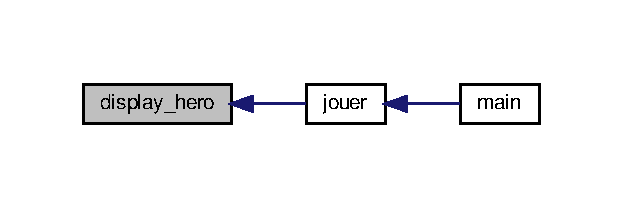
\includegraphics[width=299pt]{hero_8c_a5ed7845fc23601c05b518e32b72edc45_icgraph}
\end{center}
\end{figure}
\mbox{\Hypertarget{hero_8c_a72d8438912e0fab3e100d52b2560845e}\label{hero_8c_a72d8438912e0fab3e100d52b2560845e}} 
\index{hero.\+c@{hero.\+c}!free\+Hero@{free\+Hero}}
\index{free\+Hero@{free\+Hero}!hero.\+c@{hero.\+c}}
\subsubsection{\texorpdfstring{free\+Hero()}{freeHero()}}
{\footnotesize\ttfamily void free\+Hero (\begin{DoxyParamCaption}\item[{\hyperlink{hero_8h_aea2a78936086ab032e9479a22f656a5a}{Hero} $\ast$}]{H }\end{DoxyParamCaption})}

Here is the caller graph for this function\+:
\nopagebreak
\begin{figure}[H]
\begin{center}
\leavevmode
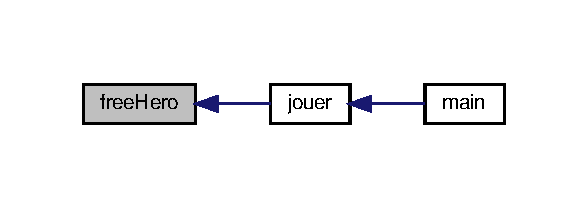
\includegraphics[width=282pt]{hero_8c_a72d8438912e0fab3e100d52b2560845e_icgraph}
\end{center}
\end{figure}
\mbox{\Hypertarget{hero_8c_a02de6fcfc96882d79393b481b079c8d3}\label{hero_8c_a02de6fcfc96882d79393b481b079c8d3}} 
\index{hero.\+c@{hero.\+c}!init\+\_\+hero@{init\+\_\+hero}}
\index{init\+\_\+hero@{init\+\_\+hero}!hero.\+c@{hero.\+c}}
\subsubsection{\texorpdfstring{init\+\_\+hero()}{init\_hero()}}
{\footnotesize\ttfamily int init\+\_\+hero (\begin{DoxyParamCaption}\item[{\hyperlink{hero_8h_aea2a78936086ab032e9479a22f656a5a}{Hero} $\ast$}]{H,  }\item[{char $\ast$}]{path }\end{DoxyParamCaption})}

Here is the call graph for this function\+:
\nopagebreak
\begin{figure}[H]
\begin{center}
\leavevmode
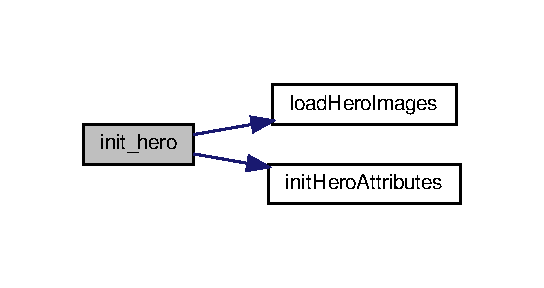
\includegraphics[width=261pt]{hero_8c_a02de6fcfc96882d79393b481b079c8d3_cgraph}
\end{center}
\end{figure}
Here is the caller graph for this function\+:
\nopagebreak
\begin{figure}[H]
\begin{center}
\leavevmode
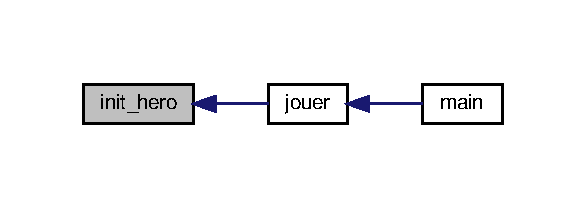
\includegraphics[width=281pt]{hero_8c_a02de6fcfc96882d79393b481b079c8d3_icgraph}
\end{center}
\end{figure}
\mbox{\Hypertarget{hero_8c_afb70c3dc1353ca52fb962b1b5e341257}\label{hero_8c_afb70c3dc1353ca52fb962b1b5e341257}} 
\index{hero.\+c@{hero.\+c}!init\+Hero\+Attributes@{init\+Hero\+Attributes}}
\index{init\+Hero\+Attributes@{init\+Hero\+Attributes}!hero.\+c@{hero.\+c}}
\subsubsection{\texorpdfstring{init\+Hero\+Attributes()}{initHeroAttributes()}}
{\footnotesize\ttfamily void init\+Hero\+Attributes (\begin{DoxyParamCaption}\item[{\hyperlink{hero_8h_aea2a78936086ab032e9479a22f656a5a}{Hero} $\ast$}]{H }\end{DoxyParamCaption})}

Here is the caller graph for this function\+:
\nopagebreak
\begin{figure}[H]
\begin{center}
\leavevmode
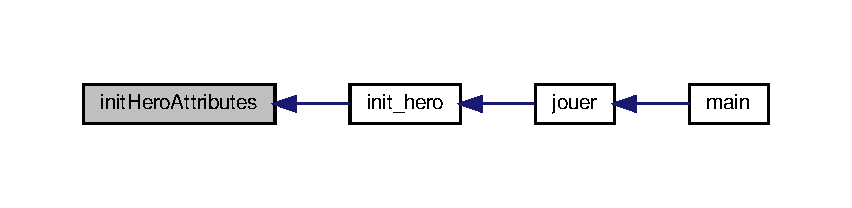
\includegraphics[width=350pt]{hero_8c_afb70c3dc1353ca52fb962b1b5e341257_icgraph}
\end{center}
\end{figure}
\mbox{\Hypertarget{hero_8c_ae11170e307c1823f644a0ed6c4fcb3d3}\label{hero_8c_ae11170e307c1823f644a0ed6c4fcb3d3}} 
\index{hero.\+c@{hero.\+c}!load\+Hero\+Images@{load\+Hero\+Images}}
\index{load\+Hero\+Images@{load\+Hero\+Images}!hero.\+c@{hero.\+c}}
\subsubsection{\texorpdfstring{load\+Hero\+Images()}{loadHeroImages()}}
{\footnotesize\ttfamily int load\+Hero\+Images (\begin{DoxyParamCaption}\item[{\hyperlink{hero_8h_aea2a78936086ab032e9479a22f656a5a}{Hero} $\ast$}]{H,  }\item[{char $\ast$}]{path }\end{DoxyParamCaption})}

Here is the caller graph for this function\+:
\nopagebreak
\begin{figure}[H]
\begin{center}
\leavevmode
\includegraphics[width=350pt]{hero_8c_ae11170e307c1823f644a0ed6c4fcb3d3_icgraph}
\end{center}
\end{figure}
\mbox{\Hypertarget{hero_8c_a949611862d28f49bddbb4db1bf587ebe}\label{hero_8c_a949611862d28f49bddbb4db1bf587ebe}} 
\index{hero.\+c@{hero.\+c}!move\+Hero@{move\+Hero}}
\index{move\+Hero@{move\+Hero}!hero.\+c@{hero.\+c}}
\subsubsection{\texorpdfstring{move\+Hero()}{moveHero()}}
{\footnotesize\ttfamily void move\+Hero (\begin{DoxyParamCaption}\item[{\hyperlink{hero_8h_aea2a78936086ab032e9479a22f656a5a}{Hero} $\ast$}]{H,  }\item[{int}]{Tab\+\_\+input\mbox{[}$\,$\mbox{]} }\end{DoxyParamCaption})}

Here is the caller graph for this function\+:
\nopagebreak
\begin{figure}[H]
\begin{center}
\leavevmode
\includegraphics[width=350pt]{hero_8c_a949611862d28f49bddbb4db1bf587ebe_icgraph}
\end{center}
\end{figure}
\mbox{\Hypertarget{hero_8c_a8d9990c46b5900c912fc96d4b091999f}\label{hero_8c_a8d9990c46b5900c912fc96d4b091999f}} 
\index{hero.\+c@{hero.\+c}!update\+\_\+hero@{update\+\_\+hero}}
\index{update\+\_\+hero@{update\+\_\+hero}!hero.\+c@{hero.\+c}}
\subsubsection{\texorpdfstring{update\+\_\+hero()}{update\_hero()}}
{\footnotesize\ttfamily void update\+\_\+hero (\begin{DoxyParamCaption}\item[{\hyperlink{hero_8h_aea2a78936086ab032e9479a22f656a5a}{Hero} $\ast$}]{H,  }\item[{int}]{Tab\+\_\+input\mbox{[}$\,$\mbox{]},  }\item[{int}]{H\+E\+\_\+collision }\end{DoxyParamCaption})}

Here is the call graph for this function\+:
\nopagebreak
\begin{figure}[H]
\begin{center}
\leavevmode
\includegraphics[width=278pt]{hero_8c_a8d9990c46b5900c912fc96d4b091999f_cgraph}
\end{center}
\end{figure}
Here is the caller graph for this function\+:
\nopagebreak
\begin{figure}[H]
\begin{center}
\leavevmode
\includegraphics[width=298pt]{hero_8c_a8d9990c46b5900c912fc96d4b091999f_icgraph}
\end{center}
\end{figure}
\mbox{\Hypertarget{hero_8c_a219651f087e4676983a70d84e7f79f13}\label{hero_8c_a219651f087e4676983a70d84e7f79f13}} 
\index{hero.\+c@{hero.\+c}!update\+Hero\+Score@{update\+Hero\+Score}}
\index{update\+Hero\+Score@{update\+Hero\+Score}!hero.\+c@{hero.\+c}}
\subsubsection{\texorpdfstring{update\+Hero\+Score()}{updateHeroScore()}}
{\footnotesize\ttfamily void update\+Hero\+Score (\begin{DoxyParamCaption}\item[{\hyperlink{hero_8h_aea2a78936086ab032e9479a22f656a5a}{Hero} $\ast$}]{H,  }\item[{int}]{H\+E\+\_\+collision }\end{DoxyParamCaption})}

Here is the caller graph for this function\+:
\nopagebreak
\begin{figure}[H]
\begin{center}
\leavevmode
\includegraphics[width=350pt]{hero_8c_a219651f087e4676983a70d84e7f79f13_icgraph}
\end{center}
\end{figure}

\hypertarget{hero_8h}{}\section{hero.\+h File Reference}
\label{hero_8h}\index{hero.\+h@{hero.\+h}}
{\ttfamily \#include $<$S\+D\+L/\+S\+D\+L.\+h$>$}\newline
{\ttfamily \#include $<$S\+D\+L/\+S\+D\+L\+\_\+image.\+h$>$}\newline
{\ttfamily \#include \char`\"{}background.\+h\char`\"{}}\newline
{\ttfamily \#include \char`\"{}defs.\+h\char`\"{}}\newline
Include dependency graph for hero.\+h\+:
\nopagebreak
\begin{figure}[H]
\begin{center}
\leavevmode
\includegraphics[width=302pt]{hero_8h__incl}
\end{center}
\end{figure}
This graph shows which files directly or indirectly include this file\+:
\nopagebreak
\begin{figure}[H]
\begin{center}
\leavevmode
\includegraphics[width=214pt]{hero_8h__dep__incl}
\end{center}
\end{figure}
\subsection*{Classes}
\begin{DoxyCompactItemize}
\item 
struct \hyperlink{structhero}{hero}
\end{DoxyCompactItemize}
\subsection*{Typedefs}
\begin{DoxyCompactItemize}
\item 
typedef struct \hyperlink{structhero}{hero} \hyperlink{hero_8h_aea2a78936086ab032e9479a22f656a5a}{Hero}
\end{DoxyCompactItemize}
\subsection*{Functions}
\begin{DoxyCompactItemize}
\item 
int \hyperlink{hero_8h_a02de6fcfc96882d79393b481b079c8d3}{init\+\_\+hero} (\hyperlink{hero_8h_aea2a78936086ab032e9479a22f656a5a}{Hero} $\ast$H, char $\ast$path)
\item 
void \hyperlink{hero_8h_a8d9990c46b5900c912fc96d4b091999f}{update\+\_\+hero} (\hyperlink{hero_8h_aea2a78936086ab032e9479a22f656a5a}{Hero} $\ast$H, int Tab\+\_\+input\mbox{[}$\,$\mbox{]}, int H\+E\+\_\+collision)
\item 
void \hyperlink{hero_8h_a5ed7845fc23601c05b518e32b72edc45}{display\+\_\+hero} (\hyperlink{hero_8h_aea2a78936086ab032e9479a22f656a5a}{Hero} H, S\+D\+L\+\_\+\+Surface $\ast$screen)
\item 
void \hyperlink{hero_8h_a72d8438912e0fab3e100d52b2560845e}{free\+Hero} (\hyperlink{hero_8h_aea2a78936086ab032e9479a22f656a5a}{Hero} $\ast$H)
\item 
int \hyperlink{hero_8h_ae11170e307c1823f644a0ed6c4fcb3d3}{load\+Hero\+Images} (\hyperlink{hero_8h_aea2a78936086ab032e9479a22f656a5a}{Hero} $\ast$H, char $\ast$path)
\item 
void \hyperlink{hero_8h_afb70c3dc1353ca52fb962b1b5e341257}{init\+Hero\+Attributes} (\hyperlink{hero_8h_aea2a78936086ab032e9479a22f656a5a}{Hero} $\ast$H)
\item 
void \hyperlink{hero_8h_a19b2ddbd3df2e9dd40de2dd5b5f33d37}{animate\+Hero} (\hyperlink{hero_8h_aea2a78936086ab032e9479a22f656a5a}{Hero} $\ast$H, int Tab\+\_\+input\mbox{[}$\,$\mbox{]}, int H\+E\+\_\+collision)
\item 
void \hyperlink{hero_8h_a949611862d28f49bddbb4db1bf587ebe}{move\+Hero} (\hyperlink{hero_8h_aea2a78936086ab032e9479a22f656a5a}{Hero} $\ast$H, int Tab\+\_\+input\mbox{[}$\,$\mbox{]})
\item 
void \hyperlink{hero_8h_a219651f087e4676983a70d84e7f79f13}{update\+Hero\+Score} (\hyperlink{hero_8h_aea2a78936086ab032e9479a22f656a5a}{Hero} $\ast$H, int H\+E\+\_\+collision)
\end{DoxyCompactItemize}


\subsection{Typedef Documentation}
\mbox{\Hypertarget{hero_8h_aea2a78936086ab032e9479a22f656a5a}\label{hero_8h_aea2a78936086ab032e9479a22f656a5a}} 
\index{hero.\+h@{hero.\+h}!Hero@{Hero}}
\index{Hero@{Hero}!hero.\+h@{hero.\+h}}
\subsubsection{\texorpdfstring{Hero}{Hero}}
{\footnotesize\ttfamily typedef struct \hyperlink{structhero}{hero} \hyperlink{hero_8h_aea2a78936086ab032e9479a22f656a5a}{Hero}}



\subsection{Function Documentation}
\mbox{\Hypertarget{hero_8h_a19b2ddbd3df2e9dd40de2dd5b5f33d37}\label{hero_8h_a19b2ddbd3df2e9dd40de2dd5b5f33d37}} 
\index{hero.\+h@{hero.\+h}!animate\+Hero@{animate\+Hero}}
\index{animate\+Hero@{animate\+Hero}!hero.\+h@{hero.\+h}}
\subsubsection{\texorpdfstring{animate\+Hero()}{animateHero()}}
{\footnotesize\ttfamily void animate\+Hero (\begin{DoxyParamCaption}\item[{\hyperlink{hero_8h_aea2a78936086ab032e9479a22f656a5a}{Hero} $\ast$}]{H,  }\item[{int}]{Tab\+\_\+input\mbox{[}$\,$\mbox{]},  }\item[{int}]{H\+E\+\_\+collision }\end{DoxyParamCaption})}

Here is the caller graph for this function\+:
\nopagebreak
\begin{figure}[H]
\begin{center}
\leavevmode
\includegraphics[width=350pt]{hero_8h_a19b2ddbd3df2e9dd40de2dd5b5f33d37_icgraph}
\end{center}
\end{figure}
\mbox{\Hypertarget{hero_8h_a5ed7845fc23601c05b518e32b72edc45}\label{hero_8h_a5ed7845fc23601c05b518e32b72edc45}} 
\index{hero.\+h@{hero.\+h}!display\+\_\+hero@{display\+\_\+hero}}
\index{display\+\_\+hero@{display\+\_\+hero}!hero.\+h@{hero.\+h}}
\subsubsection{\texorpdfstring{display\+\_\+hero()}{display\_hero()}}
{\footnotesize\ttfamily void display\+\_\+hero (\begin{DoxyParamCaption}\item[{\hyperlink{hero_8h_aea2a78936086ab032e9479a22f656a5a}{Hero}}]{H,  }\item[{S\+D\+L\+\_\+\+Surface $\ast$}]{screen }\end{DoxyParamCaption})}

Here is the caller graph for this function\+:
\nopagebreak
\begin{figure}[H]
\begin{center}
\leavevmode
\includegraphics[width=299pt]{hero_8h_a5ed7845fc23601c05b518e32b72edc45_icgraph}
\end{center}
\end{figure}
\mbox{\Hypertarget{hero_8h_a72d8438912e0fab3e100d52b2560845e}\label{hero_8h_a72d8438912e0fab3e100d52b2560845e}} 
\index{hero.\+h@{hero.\+h}!free\+Hero@{free\+Hero}}
\index{free\+Hero@{free\+Hero}!hero.\+h@{hero.\+h}}
\subsubsection{\texorpdfstring{free\+Hero()}{freeHero()}}
{\footnotesize\ttfamily void free\+Hero (\begin{DoxyParamCaption}\item[{\hyperlink{hero_8h_aea2a78936086ab032e9479a22f656a5a}{Hero} $\ast$}]{H }\end{DoxyParamCaption})}

Here is the caller graph for this function\+:
\nopagebreak
\begin{figure}[H]
\begin{center}
\leavevmode
\includegraphics[width=282pt]{hero_8h_a72d8438912e0fab3e100d52b2560845e_icgraph}
\end{center}
\end{figure}
\mbox{\Hypertarget{hero_8h_a02de6fcfc96882d79393b481b079c8d3}\label{hero_8h_a02de6fcfc96882d79393b481b079c8d3}} 
\index{hero.\+h@{hero.\+h}!init\+\_\+hero@{init\+\_\+hero}}
\index{init\+\_\+hero@{init\+\_\+hero}!hero.\+h@{hero.\+h}}
\subsubsection{\texorpdfstring{init\+\_\+hero()}{init\_hero()}}
{\footnotesize\ttfamily int init\+\_\+hero (\begin{DoxyParamCaption}\item[{\hyperlink{hero_8h_aea2a78936086ab032e9479a22f656a5a}{Hero} $\ast$}]{H,  }\item[{char $\ast$}]{path }\end{DoxyParamCaption})}

Here is the call graph for this function\+:
\nopagebreak
\begin{figure}[H]
\begin{center}
\leavevmode
\includegraphics[width=261pt]{hero_8h_a02de6fcfc96882d79393b481b079c8d3_cgraph}
\end{center}
\end{figure}
Here is the caller graph for this function\+:
\nopagebreak
\begin{figure}[H]
\begin{center}
\leavevmode
\includegraphics[width=281pt]{hero_8h_a02de6fcfc96882d79393b481b079c8d3_icgraph}
\end{center}
\end{figure}
\mbox{\Hypertarget{hero_8h_afb70c3dc1353ca52fb962b1b5e341257}\label{hero_8h_afb70c3dc1353ca52fb962b1b5e341257}} 
\index{hero.\+h@{hero.\+h}!init\+Hero\+Attributes@{init\+Hero\+Attributes}}
\index{init\+Hero\+Attributes@{init\+Hero\+Attributes}!hero.\+h@{hero.\+h}}
\subsubsection{\texorpdfstring{init\+Hero\+Attributes()}{initHeroAttributes()}}
{\footnotesize\ttfamily void init\+Hero\+Attributes (\begin{DoxyParamCaption}\item[{\hyperlink{hero_8h_aea2a78936086ab032e9479a22f656a5a}{Hero} $\ast$}]{H }\end{DoxyParamCaption})}

Here is the caller graph for this function\+:
\nopagebreak
\begin{figure}[H]
\begin{center}
\leavevmode
\includegraphics[width=350pt]{hero_8h_afb70c3dc1353ca52fb962b1b5e341257_icgraph}
\end{center}
\end{figure}
\mbox{\Hypertarget{hero_8h_ae11170e307c1823f644a0ed6c4fcb3d3}\label{hero_8h_ae11170e307c1823f644a0ed6c4fcb3d3}} 
\index{hero.\+h@{hero.\+h}!load\+Hero\+Images@{load\+Hero\+Images}}
\index{load\+Hero\+Images@{load\+Hero\+Images}!hero.\+h@{hero.\+h}}
\subsubsection{\texorpdfstring{load\+Hero\+Images()}{loadHeroImages()}}
{\footnotesize\ttfamily int load\+Hero\+Images (\begin{DoxyParamCaption}\item[{\hyperlink{hero_8h_aea2a78936086ab032e9479a22f656a5a}{Hero} $\ast$}]{H,  }\item[{char $\ast$}]{path }\end{DoxyParamCaption})}

Here is the caller graph for this function\+:
\nopagebreak
\begin{figure}[H]
\begin{center}
\leavevmode
\includegraphics[width=350pt]{hero_8h_ae11170e307c1823f644a0ed6c4fcb3d3_icgraph}
\end{center}
\end{figure}
\mbox{\Hypertarget{hero_8h_a949611862d28f49bddbb4db1bf587ebe}\label{hero_8h_a949611862d28f49bddbb4db1bf587ebe}} 
\index{hero.\+h@{hero.\+h}!move\+Hero@{move\+Hero}}
\index{move\+Hero@{move\+Hero}!hero.\+h@{hero.\+h}}
\subsubsection{\texorpdfstring{move\+Hero()}{moveHero()}}
{\footnotesize\ttfamily void move\+Hero (\begin{DoxyParamCaption}\item[{\hyperlink{hero_8h_aea2a78936086ab032e9479a22f656a5a}{Hero} $\ast$}]{H,  }\item[{int}]{Tab\+\_\+input\mbox{[}$\,$\mbox{]} }\end{DoxyParamCaption})}

Here is the caller graph for this function\+:
\nopagebreak
\begin{figure}[H]
\begin{center}
\leavevmode
\includegraphics[width=350pt]{hero_8h_a949611862d28f49bddbb4db1bf587ebe_icgraph}
\end{center}
\end{figure}
\mbox{\Hypertarget{hero_8h_a8d9990c46b5900c912fc96d4b091999f}\label{hero_8h_a8d9990c46b5900c912fc96d4b091999f}} 
\index{hero.\+h@{hero.\+h}!update\+\_\+hero@{update\+\_\+hero}}
\index{update\+\_\+hero@{update\+\_\+hero}!hero.\+h@{hero.\+h}}
\subsubsection{\texorpdfstring{update\+\_\+hero()}{update\_hero()}}
{\footnotesize\ttfamily void update\+\_\+hero (\begin{DoxyParamCaption}\item[{\hyperlink{hero_8h_aea2a78936086ab032e9479a22f656a5a}{Hero} $\ast$}]{H,  }\item[{int}]{Tab\+\_\+input\mbox{[}$\,$\mbox{]},  }\item[{int}]{H\+E\+\_\+collision }\end{DoxyParamCaption})}

Here is the call graph for this function\+:
\nopagebreak
\begin{figure}[H]
\begin{center}
\leavevmode
\includegraphics[width=278pt]{hero_8h_a8d9990c46b5900c912fc96d4b091999f_cgraph}
\end{center}
\end{figure}
Here is the caller graph for this function\+:
\nopagebreak
\begin{figure}[H]
\begin{center}
\leavevmode
\includegraphics[width=298pt]{hero_8h_a8d9990c46b5900c912fc96d4b091999f_icgraph}
\end{center}
\end{figure}
\mbox{\Hypertarget{hero_8h_a219651f087e4676983a70d84e7f79f13}\label{hero_8h_a219651f087e4676983a70d84e7f79f13}} 
\index{hero.\+h@{hero.\+h}!update\+Hero\+Score@{update\+Hero\+Score}}
\index{update\+Hero\+Score@{update\+Hero\+Score}!hero.\+h@{hero.\+h}}
\subsubsection{\texorpdfstring{update\+Hero\+Score()}{updateHeroScore()}}
{\footnotesize\ttfamily void update\+Hero\+Score (\begin{DoxyParamCaption}\item[{\hyperlink{hero_8h_aea2a78936086ab032e9479a22f656a5a}{Hero} $\ast$}]{H,  }\item[{int}]{H\+E\+\_\+collision }\end{DoxyParamCaption})}

Here is the caller graph for this function\+:
\nopagebreak
\begin{figure}[H]
\begin{center}
\leavevmode
\includegraphics[width=350pt]{hero_8h_a219651f087e4676983a70d84e7f79f13_icgraph}
\end{center}
\end{figure}

\hypertarget{jeu_8c}{}\section{jeu.\+c File Reference}
\label{jeu_8c}\index{jeu.\+c@{jeu.\+c}}
{\ttfamily \#include \char`\"{}jeu.\+h\char`\"{}}\newline
Include dependency graph for jeu.\+c\+:
\nopagebreak
\begin{figure}[H]
\begin{center}
\leavevmode
\includegraphics[width=350pt]{jeu_8c__incl}
\end{center}
\end{figure}
\subsection*{Functions}
\begin{DoxyCompactItemize}
\item 
void \hyperlink{jeu_8c_a0042a71e38e225e5874875d59387dfbe}{get\+\_\+input} (int Tab\+\_\+input\mbox{[}$\,$\mbox{]}, S\+D\+L\+\_\+\+Event event)
\item 
int \hyperlink{jeu_8c_ad9c436fc5815440f57648231b18e2caf}{jouer} (S\+D\+L\+\_\+\+Surface $\ast$screen)
\end{DoxyCompactItemize}


\subsection{Function Documentation}
\mbox{\Hypertarget{jeu_8c_a0042a71e38e225e5874875d59387dfbe}\label{jeu_8c_a0042a71e38e225e5874875d59387dfbe}} 
\index{jeu.\+c@{jeu.\+c}!get\+\_\+input@{get\+\_\+input}}
\index{get\+\_\+input@{get\+\_\+input}!jeu.\+c@{jeu.\+c}}
\subsubsection{\texorpdfstring{get\+\_\+input()}{get\_input()}}
{\footnotesize\ttfamily void get\+\_\+input (\begin{DoxyParamCaption}\item[{int}]{Tab\+\_\+input\mbox{[}$\,$\mbox{]},  }\item[{S\+D\+L\+\_\+\+Event}]{event }\end{DoxyParamCaption})}

Here is the caller graph for this function\+:
\nopagebreak
\begin{figure}[H]
\begin{center}
\leavevmode
\includegraphics[width=284pt]{jeu_8c_a0042a71e38e225e5874875d59387dfbe_icgraph}
\end{center}
\end{figure}
\mbox{\Hypertarget{jeu_8c_ad9c436fc5815440f57648231b18e2caf}\label{jeu_8c_ad9c436fc5815440f57648231b18e2caf}} 
\index{jeu.\+c@{jeu.\+c}!jouer@{jouer}}
\index{jouer@{jouer}!jeu.\+c@{jeu.\+c}}
\subsubsection{\texorpdfstring{jouer()}{jouer()}}
{\footnotesize\ttfamily int jouer (\begin{DoxyParamCaption}\item[{S\+D\+L\+\_\+\+Surface $\ast$}]{screen }\end{DoxyParamCaption})}

Here is the call graph for this function\+:
\nopagebreak
\begin{figure}[H]
\begin{center}
\leavevmode
\includegraphics[height=550pt]{jeu_8c_ad9c436fc5815440f57648231b18e2caf_cgraph}
\end{center}
\end{figure}
Here is the caller graph for this function\+:
\nopagebreak
\begin{figure}[H]
\begin{center}
\leavevmode
\includegraphics[width=192pt]{jeu_8c_ad9c436fc5815440f57648231b18e2caf_icgraph}
\end{center}
\end{figure}

\hypertarget{jeu_8h}{}\section{jeu.\+h File Reference}
\label{jeu_8h}\index{jeu.\+h@{jeu.\+h}}
{\ttfamily \#include $<$S\+D\+L/\+S\+D\+L.\+h$>$}\newline
{\ttfamily \#include \char`\"{}defs.\+h\char`\"{}}\newline
{\ttfamily \#include \char`\"{}background.\+h\char`\"{}}\newline
{\ttfamily \#include \char`\"{}ennemi.\+h\char`\"{}}\newline
{\ttfamily \#include \char`\"{}hero.\+h\char`\"{}}\newline
{\ttfamily \#include \char`\"{}text.\+h\char`\"{}}\newline
Include dependency graph for jeu.\+h\+:
\nopagebreak
\begin{figure}[H]
\begin{center}
\leavevmode
\includegraphics[width=350pt]{jeu_8h__incl}
\end{center}
\end{figure}
This graph shows which files directly or indirectly include this file\+:
\nopagebreak
\begin{figure}[H]
\begin{center}
\leavevmode
\includegraphics[width=182pt]{jeu_8h__dep__incl}
\end{center}
\end{figure}
\subsection*{Functions}
\begin{DoxyCompactItemize}
\item 
void \hyperlink{jeu_8h_a0042a71e38e225e5874875d59387dfbe}{get\+\_\+input} (int Tab\+\_\+input\mbox{[}$\,$\mbox{]}, S\+D\+L\+\_\+\+Event event)
\item 
int \hyperlink{jeu_8h_ad9c436fc5815440f57648231b18e2caf}{jouer} (S\+D\+L\+\_\+\+Surface $\ast$screen)
\end{DoxyCompactItemize}


\subsection{Function Documentation}
\mbox{\Hypertarget{jeu_8h_a0042a71e38e225e5874875d59387dfbe}\label{jeu_8h_a0042a71e38e225e5874875d59387dfbe}} 
\index{jeu.\+h@{jeu.\+h}!get\+\_\+input@{get\+\_\+input}}
\index{get\+\_\+input@{get\+\_\+input}!jeu.\+h@{jeu.\+h}}
\subsubsection{\texorpdfstring{get\+\_\+input()}{get\_input()}}
{\footnotesize\ttfamily void get\+\_\+input (\begin{DoxyParamCaption}\item[{int}]{Tab\+\_\+input\mbox{[}$\,$\mbox{]},  }\item[{S\+D\+L\+\_\+\+Event}]{event }\end{DoxyParamCaption})}

Here is the caller graph for this function\+:
\nopagebreak
\begin{figure}[H]
\begin{center}
\leavevmode
\includegraphics[width=284pt]{jeu_8h_a0042a71e38e225e5874875d59387dfbe_icgraph}
\end{center}
\end{figure}
\mbox{\Hypertarget{jeu_8h_ad9c436fc5815440f57648231b18e2caf}\label{jeu_8h_ad9c436fc5815440f57648231b18e2caf}} 
\index{jeu.\+h@{jeu.\+h}!jouer@{jouer}}
\index{jouer@{jouer}!jeu.\+h@{jeu.\+h}}
\subsubsection{\texorpdfstring{jouer()}{jouer()}}
{\footnotesize\ttfamily int jouer (\begin{DoxyParamCaption}\item[{S\+D\+L\+\_\+\+Surface $\ast$}]{screen }\end{DoxyParamCaption})}

Here is the call graph for this function\+:
\nopagebreak
\begin{figure}[H]
\begin{center}
\leavevmode
\includegraphics[height=550pt]{jeu_8h_ad9c436fc5815440f57648231b18e2caf_cgraph}
\end{center}
\end{figure}
Here is the caller graph for this function\+:
\nopagebreak
\begin{figure}[H]
\begin{center}
\leavevmode
\includegraphics[width=192pt]{jeu_8h_ad9c436fc5815440f57648231b18e2caf_icgraph}
\end{center}
\end{figure}

\hypertarget{main_8c}{}\section{main.\+c File Reference}
\label{main_8c}\index{main.\+c@{main.\+c}}
{\ttfamily \#include $<$stdio.\+h$>$}\newline
{\ttfamily \#include $<$stdlib.\+h$>$}\newline
{\ttfamily \#include $<$S\+D\+L/\+S\+D\+L.\+h$>$}\newline
{\ttfamily \#include $<$S\+D\+L/\+S\+D\+L\+\_\+image.\+h$>$}\newline
{\ttfamily \#include $<$S\+D\+L/\+S\+D\+L\+\_\+ttf.\+h$>$}\newline
{\ttfamily \#include \char`\"{}S\+D\+L/\+S\+D\+L\+\_\+mixer.\+h\char`\"{}}\newline
{\ttfamily \#include \char`\"{}menu.\+h\char`\"{}}\newline
Include dependency graph for main.\+c\+:
\nopagebreak
\begin{figure}[H]
\begin{center}
\leavevmode
\includegraphics[width=350pt]{main_8c__incl}
\end{center}
\end{figure}
\subsection*{Functions}
\begin{DoxyCompactItemize}
\item 
int \hyperlink{main_8c_ae66f6b31b5ad750f1fe042a706a4e3d4}{main} ()
\end{DoxyCompactItemize}


\subsection{Function Documentation}
\mbox{\Hypertarget{main_8c_ae66f6b31b5ad750f1fe042a706a4e3d4}\label{main_8c_ae66f6b31b5ad750f1fe042a706a4e3d4}} 
\index{main.\+c@{main.\+c}!main@{main}}
\index{main@{main}!main.\+c@{main.\+c}}
\subsubsection{\texorpdfstring{main()}{main()}}
{\footnotesize\ttfamily int main (\begin{DoxyParamCaption}{ }\end{DoxyParamCaption})}

Here is the call graph for this function\+:
\nopagebreak
\begin{figure}[H]
\begin{center}
\leavevmode
\includegraphics[width=350pt]{main_8c_ae66f6b31b5ad750f1fe042a706a4e3d4_cgraph}
\end{center}
\end{figure}

\hypertarget{text_8c}{}\section{text.\+c File Reference}
\label{text_8c}\index{text.\+c@{text.\+c}}
{\ttfamily \#include \char`\"{}text.\+h\char`\"{}}\newline
Include dependency graph for text.\+c\+:
\nopagebreak
\begin{figure}[H]
\begin{center}
\leavevmode
\includegraphics[width=313pt]{text_8c__incl}
\end{center}
\end{figure}
\subsection*{Functions}
\begin{DoxyCompactItemize}
\item 
int \hyperlink{text_8c_ac269a46f79e51608ef78cd4cb1c45ce2}{init\+\_\+text} (\hyperlink{text_8h_ae244dd94cd8740c225560d14fb17e508}{Text} $\ast$T, char $\ast$path)
\item 
int \hyperlink{text_8c_aaeca0de4db7b2b3adab7953e103ab254}{load\+Font} (\hyperlink{text_8h_ae244dd94cd8740c225560d14fb17e508}{Text} $\ast$T, char $\ast$path)
\item 
void \hyperlink{text_8c_a0ea79d8f0ab786ff1512f02154b8615f}{init\+Text\+Attributes} (\hyperlink{text_8h_ae244dd94cd8740c225560d14fb17e508}{Text} $\ast$T)
\item 
void \hyperlink{text_8c_a2a40daca85de6bc00538e32c91d4220e}{update\+\_\+txt} (\hyperlink{text_8h_ae244dd94cd8740c225560d14fb17e508}{Text} $\ast$T, int vies\+Hero)
\item 
void \hyperlink{text_8c_acdafc8b8de5b1a0309c13c3fe4cf9a8a}{display\+Text} (\hyperlink{text_8h_ae244dd94cd8740c225560d14fb17e508}{Text} T, S\+D\+L\+\_\+\+Surface $\ast$screen)
\item 
void \hyperlink{text_8c_aa642dcc238a888eacbb2c80a3f604ee1}{free\+Text} (\hyperlink{text_8h_ae244dd94cd8740c225560d14fb17e508}{Text} $\ast$T)
\end{DoxyCompactItemize}


\subsection{Function Documentation}
\mbox{\Hypertarget{text_8c_acdafc8b8de5b1a0309c13c3fe4cf9a8a}\label{text_8c_acdafc8b8de5b1a0309c13c3fe4cf9a8a}} 
\index{text.\+c@{text.\+c}!display\+Text@{display\+Text}}
\index{display\+Text@{display\+Text}!text.\+c@{text.\+c}}
\subsubsection{\texorpdfstring{display\+Text()}{displayText()}}
{\footnotesize\ttfamily void display\+Text (\begin{DoxyParamCaption}\item[{\hyperlink{text_8h_ae244dd94cd8740c225560d14fb17e508}{Text}}]{T,  }\item[{S\+D\+L\+\_\+\+Surface $\ast$}]{screen }\end{DoxyParamCaption})}

Here is the caller graph for this function\+:
\nopagebreak
\begin{figure}[H]
\begin{center}
\leavevmode
\includegraphics[width=295pt]{text_8c_acdafc8b8de5b1a0309c13c3fe4cf9a8a_icgraph}
\end{center}
\end{figure}
\mbox{\Hypertarget{text_8c_aa642dcc238a888eacbb2c80a3f604ee1}\label{text_8c_aa642dcc238a888eacbb2c80a3f604ee1}} 
\index{text.\+c@{text.\+c}!free\+Text@{free\+Text}}
\index{free\+Text@{free\+Text}!text.\+c@{text.\+c}}
\subsubsection{\texorpdfstring{free\+Text()}{freeText()}}
{\footnotesize\ttfamily void free\+Text (\begin{DoxyParamCaption}\item[{\hyperlink{text_8h_ae244dd94cd8740c225560d14fb17e508}{Text} $\ast$}]{T }\end{DoxyParamCaption})}

Here is the caller graph for this function\+:
\nopagebreak
\begin{figure}[H]
\begin{center}
\leavevmode
\includegraphics[width=281pt]{text_8c_aa642dcc238a888eacbb2c80a3f604ee1_icgraph}
\end{center}
\end{figure}
\mbox{\Hypertarget{text_8c_ac269a46f79e51608ef78cd4cb1c45ce2}\label{text_8c_ac269a46f79e51608ef78cd4cb1c45ce2}} 
\index{text.\+c@{text.\+c}!init\+\_\+text@{init\+\_\+text}}
\index{init\+\_\+text@{init\+\_\+text}!text.\+c@{text.\+c}}
\subsubsection{\texorpdfstring{init\+\_\+text()}{init\_text()}}
{\footnotesize\ttfamily int init\+\_\+text (\begin{DoxyParamCaption}\item[{\hyperlink{text_8h_ae244dd94cd8740c225560d14fb17e508}{Text} $\ast$}]{T,  }\item[{char $\ast$}]{path }\end{DoxyParamCaption})}

Here is the call graph for this function\+:
\nopagebreak
\begin{figure}[H]
\begin{center}
\leavevmode
\includegraphics[width=258pt]{text_8c_ac269a46f79e51608ef78cd4cb1c45ce2_cgraph}
\end{center}
\end{figure}
Here is the caller graph for this function\+:
\nopagebreak
\begin{figure}[H]
\begin{center}
\leavevmode
\includegraphics[width=279pt]{text_8c_ac269a46f79e51608ef78cd4cb1c45ce2_icgraph}
\end{center}
\end{figure}
\mbox{\Hypertarget{text_8c_a0ea79d8f0ab786ff1512f02154b8615f}\label{text_8c_a0ea79d8f0ab786ff1512f02154b8615f}} 
\index{text.\+c@{text.\+c}!init\+Text\+Attributes@{init\+Text\+Attributes}}
\index{init\+Text\+Attributes@{init\+Text\+Attributes}!text.\+c@{text.\+c}}
\subsubsection{\texorpdfstring{init\+Text\+Attributes()}{initTextAttributes()}}
{\footnotesize\ttfamily void init\+Text\+Attributes (\begin{DoxyParamCaption}\item[{\hyperlink{text_8h_ae244dd94cd8740c225560d14fb17e508}{Text} $\ast$}]{T }\end{DoxyParamCaption})}

Here is the caller graph for this function\+:
\nopagebreak
\begin{figure}[H]
\begin{center}
\leavevmode
\includegraphics[width=350pt]{text_8c_a0ea79d8f0ab786ff1512f02154b8615f_icgraph}
\end{center}
\end{figure}
\mbox{\Hypertarget{text_8c_aaeca0de4db7b2b3adab7953e103ab254}\label{text_8c_aaeca0de4db7b2b3adab7953e103ab254}} 
\index{text.\+c@{text.\+c}!load\+Font@{load\+Font}}
\index{load\+Font@{load\+Font}!text.\+c@{text.\+c}}
\subsubsection{\texorpdfstring{load\+Font()}{loadFont()}}
{\footnotesize\ttfamily int load\+Font (\begin{DoxyParamCaption}\item[{\hyperlink{text_8h_ae244dd94cd8740c225560d14fb17e508}{Text} $\ast$}]{T,  }\item[{char $\ast$}]{path }\end{DoxyParamCaption})}

Here is the caller graph for this function\+:
\nopagebreak
\begin{figure}[H]
\begin{center}
\leavevmode
\includegraphics[width=350pt]{text_8c_aaeca0de4db7b2b3adab7953e103ab254_icgraph}
\end{center}
\end{figure}
\mbox{\Hypertarget{text_8c_a2a40daca85de6bc00538e32c91d4220e}\label{text_8c_a2a40daca85de6bc00538e32c91d4220e}} 
\index{text.\+c@{text.\+c}!update\+\_\+txt@{update\+\_\+txt}}
\index{update\+\_\+txt@{update\+\_\+txt}!text.\+c@{text.\+c}}
\subsubsection{\texorpdfstring{update\+\_\+txt()}{update\_txt()}}
{\footnotesize\ttfamily void update\+\_\+txt (\begin{DoxyParamCaption}\item[{\hyperlink{text_8h_ae244dd94cd8740c225560d14fb17e508}{Text} $\ast$}]{T,  }\item[{int}]{vies\+Hero }\end{DoxyParamCaption})}

Here is the caller graph for this function\+:
\nopagebreak
\begin{figure}[H]
\begin{center}
\leavevmode
\includegraphics[width=290pt]{text_8c_a2a40daca85de6bc00538e32c91d4220e_icgraph}
\end{center}
\end{figure}

\hypertarget{text_8h}{}\section{text.\+h File Reference}
\label{text_8h}\index{text.\+h@{text.\+h}}
{\ttfamily \#include $<$S\+D\+L/\+S\+D\+L.\+h$>$}\newline
{\ttfamily \#include $<$S\+D\+L/\+S\+D\+L\+\_\+ttf.\+h$>$}\newline
{\ttfamily \#include $<$string.\+h$>$}\newline
Include dependency graph for text.\+h\+:
\nopagebreak
\begin{figure}[H]
\begin{center}
\leavevmode
\includegraphics[width=313pt]{text_8h__incl}
\end{center}
\end{figure}
This graph shows which files directly or indirectly include this file\+:
\nopagebreak
\begin{figure}[H]
\begin{center}
\leavevmode
\includegraphics[width=208pt]{text_8h__dep__incl}
\end{center}
\end{figure}
\subsection*{Classes}
\begin{DoxyCompactItemize}
\item 
struct \hyperlink{structtext}{text}
\end{DoxyCompactItemize}
\subsection*{Typedefs}
\begin{DoxyCompactItemize}
\item 
typedef struct \hyperlink{structtext}{text} \hyperlink{text_8h_ae244dd94cd8740c225560d14fb17e508}{Text}
\end{DoxyCompactItemize}
\subsection*{Functions}
\begin{DoxyCompactItemize}
\item 
int \hyperlink{text_8h_ac269a46f79e51608ef78cd4cb1c45ce2}{init\+\_\+text} (\hyperlink{text_8h_ae244dd94cd8740c225560d14fb17e508}{Text} $\ast$T, char $\ast$path)
\item 
void \hyperlink{text_8h_a2a40daca85de6bc00538e32c91d4220e}{update\+\_\+txt} (\hyperlink{text_8h_ae244dd94cd8740c225560d14fb17e508}{Text} $\ast$T, int vies\+Hero)
\item 
void \hyperlink{text_8h_acdafc8b8de5b1a0309c13c3fe4cf9a8a}{display\+Text} (\hyperlink{text_8h_ae244dd94cd8740c225560d14fb17e508}{Text} T, S\+D\+L\+\_\+\+Surface $\ast$screen)
\item 
void \hyperlink{text_8h_aa642dcc238a888eacbb2c80a3f604ee1}{free\+Text} (\hyperlink{text_8h_ae244dd94cd8740c225560d14fb17e508}{Text} $\ast$T)
\item 
void \hyperlink{text_8h_a0ea79d8f0ab786ff1512f02154b8615f}{init\+Text\+Attributes} (\hyperlink{text_8h_ae244dd94cd8740c225560d14fb17e508}{Text} $\ast$T)
\item 
int \hyperlink{text_8h_aaeca0de4db7b2b3adab7953e103ab254}{load\+Font} (\hyperlink{text_8h_ae244dd94cd8740c225560d14fb17e508}{Text} $\ast$T, char $\ast$path)
\end{DoxyCompactItemize}


\subsection{Typedef Documentation}
\mbox{\Hypertarget{text_8h_ae244dd94cd8740c225560d14fb17e508}\label{text_8h_ae244dd94cd8740c225560d14fb17e508}} 
\index{text.\+h@{text.\+h}!Text@{Text}}
\index{Text@{Text}!text.\+h@{text.\+h}}
\subsubsection{\texorpdfstring{Text}{Text}}
{\footnotesize\ttfamily typedef struct \hyperlink{structtext}{text} \hyperlink{text_8h_ae244dd94cd8740c225560d14fb17e508}{Text}}



\subsection{Function Documentation}
\mbox{\Hypertarget{text_8h_acdafc8b8de5b1a0309c13c3fe4cf9a8a}\label{text_8h_acdafc8b8de5b1a0309c13c3fe4cf9a8a}} 
\index{text.\+h@{text.\+h}!display\+Text@{display\+Text}}
\index{display\+Text@{display\+Text}!text.\+h@{text.\+h}}
\subsubsection{\texorpdfstring{display\+Text()}{displayText()}}
{\footnotesize\ttfamily void display\+Text (\begin{DoxyParamCaption}\item[{\hyperlink{text_8h_ae244dd94cd8740c225560d14fb17e508}{Text}}]{T,  }\item[{S\+D\+L\+\_\+\+Surface $\ast$}]{screen }\end{DoxyParamCaption})}

Here is the caller graph for this function\+:
\nopagebreak
\begin{figure}[H]
\begin{center}
\leavevmode
\includegraphics[width=295pt]{text_8h_acdafc8b8de5b1a0309c13c3fe4cf9a8a_icgraph}
\end{center}
\end{figure}
\mbox{\Hypertarget{text_8h_aa642dcc238a888eacbb2c80a3f604ee1}\label{text_8h_aa642dcc238a888eacbb2c80a3f604ee1}} 
\index{text.\+h@{text.\+h}!free\+Text@{free\+Text}}
\index{free\+Text@{free\+Text}!text.\+h@{text.\+h}}
\subsubsection{\texorpdfstring{free\+Text()}{freeText()}}
{\footnotesize\ttfamily void free\+Text (\begin{DoxyParamCaption}\item[{\hyperlink{text_8h_ae244dd94cd8740c225560d14fb17e508}{Text} $\ast$}]{T }\end{DoxyParamCaption})}

Here is the caller graph for this function\+:
\nopagebreak
\begin{figure}[H]
\begin{center}
\leavevmode
\includegraphics[width=281pt]{text_8h_aa642dcc238a888eacbb2c80a3f604ee1_icgraph}
\end{center}
\end{figure}
\mbox{\Hypertarget{text_8h_ac269a46f79e51608ef78cd4cb1c45ce2}\label{text_8h_ac269a46f79e51608ef78cd4cb1c45ce2}} 
\index{text.\+h@{text.\+h}!init\+\_\+text@{init\+\_\+text}}
\index{init\+\_\+text@{init\+\_\+text}!text.\+h@{text.\+h}}
\subsubsection{\texorpdfstring{init\+\_\+text()}{init\_text()}}
{\footnotesize\ttfamily int init\+\_\+text (\begin{DoxyParamCaption}\item[{\hyperlink{text_8h_ae244dd94cd8740c225560d14fb17e508}{Text} $\ast$}]{T,  }\item[{char $\ast$}]{path }\end{DoxyParamCaption})}

Here is the call graph for this function\+:
\nopagebreak
\begin{figure}[H]
\begin{center}
\leavevmode
\includegraphics[width=258pt]{text_8h_ac269a46f79e51608ef78cd4cb1c45ce2_cgraph}
\end{center}
\end{figure}
Here is the caller graph for this function\+:
\nopagebreak
\begin{figure}[H]
\begin{center}
\leavevmode
\includegraphics[width=279pt]{text_8h_ac269a46f79e51608ef78cd4cb1c45ce2_icgraph}
\end{center}
\end{figure}
\mbox{\Hypertarget{text_8h_a0ea79d8f0ab786ff1512f02154b8615f}\label{text_8h_a0ea79d8f0ab786ff1512f02154b8615f}} 
\index{text.\+h@{text.\+h}!init\+Text\+Attributes@{init\+Text\+Attributes}}
\index{init\+Text\+Attributes@{init\+Text\+Attributes}!text.\+h@{text.\+h}}
\subsubsection{\texorpdfstring{init\+Text\+Attributes()}{initTextAttributes()}}
{\footnotesize\ttfamily void init\+Text\+Attributes (\begin{DoxyParamCaption}\item[{\hyperlink{text_8h_ae244dd94cd8740c225560d14fb17e508}{Text} $\ast$}]{T }\end{DoxyParamCaption})}

Here is the caller graph for this function\+:
\nopagebreak
\begin{figure}[H]
\begin{center}
\leavevmode
\includegraphics[width=350pt]{text_8h_a0ea79d8f0ab786ff1512f02154b8615f_icgraph}
\end{center}
\end{figure}
\mbox{\Hypertarget{text_8h_aaeca0de4db7b2b3adab7953e103ab254}\label{text_8h_aaeca0de4db7b2b3adab7953e103ab254}} 
\index{text.\+h@{text.\+h}!load\+Font@{load\+Font}}
\index{load\+Font@{load\+Font}!text.\+h@{text.\+h}}
\subsubsection{\texorpdfstring{load\+Font()}{loadFont()}}
{\footnotesize\ttfamily int load\+Font (\begin{DoxyParamCaption}\item[{\hyperlink{text_8h_ae244dd94cd8740c225560d14fb17e508}{Text} $\ast$}]{T,  }\item[{char $\ast$}]{path }\end{DoxyParamCaption})}

Here is the caller graph for this function\+:
\nopagebreak
\begin{figure}[H]
\begin{center}
\leavevmode
\includegraphics[width=350pt]{text_8h_aaeca0de4db7b2b3adab7953e103ab254_icgraph}
\end{center}
\end{figure}
\mbox{\Hypertarget{text_8h_a2a40daca85de6bc00538e32c91d4220e}\label{text_8h_a2a40daca85de6bc00538e32c91d4220e}} 
\index{text.\+h@{text.\+h}!update\+\_\+txt@{update\+\_\+txt}}
\index{update\+\_\+txt@{update\+\_\+txt}!text.\+h@{text.\+h}}
\subsubsection{\texorpdfstring{update\+\_\+txt()}{update\_txt()}}
{\footnotesize\ttfamily void update\+\_\+txt (\begin{DoxyParamCaption}\item[{\hyperlink{text_8h_ae244dd94cd8740c225560d14fb17e508}{Text} $\ast$}]{T,  }\item[{int}]{vies\+Hero }\end{DoxyParamCaption})}

Here is the caller graph for this function\+:
\nopagebreak
\begin{figure}[H]
\begin{center}
\leavevmode
\includegraphics[width=290pt]{text_8h_a2a40daca85de6bc00538e32c91d4220e_icgraph}
\end{center}
\end{figure}

%--- End generated contents ---

% Index
\backmatter
\newpage
\phantomsection
\clearemptydoublepage
\addcontentsline{toc}{chapter}{Index}
\printindex

\end{document}
